%% bare_jrnl.tex
%% V1.4b
%% 2015/08/26
%% by Michael Shell
%% see http://www.michaelshell.org/
%% for current contact information.
%%
%% This is a skeleton file demonstrating the use of IEEEtran.cls
%% (requires IEEEtran.cls version 1.8b or later) with an IEEE
%% journal paper.
%%
%% Support sites:
%% http://www.michaelshell.org/tex/ieeetran/
%% http://www.ctan.org/pkg/ieeetran
%% and
%% http://www.ieee.org/

%%*************************************************************************
%% Legal Notice:
%% This code is offered as-is without any warranty either expressed or
%% implied; without even the implied warranty of MERCHANTABILITY or
%% FITNESS FOR A PARTICULAR PURPOSE! 
%% User assumes all risk.
%% In no event shall the IEEE or any contributor to this code be liable for
%% any damages or losses, including, but not limited to, incidental,
%% consequential, or any other damages, resulting from the use or misuse
%% of any information contained here.
%%
%% All comments are the opinions of their respective authors and are not
%% necessarily endorsed by the IEEE.
%%
%% This work is distributed under the LaTeX Project Public License (LPPL)
%% ( http://www.latex-project.org/ ) version 1.3, and may be freely used,
%% distributed and modified. A copy of the LPPL, version 1.3, is included
%% in the base LaTeX documentation of all distributions of LaTeX released
%% 2003/12/01 or later.
%% Retain all contribution notices and credits.
%% ** Modified files should be clearly indicated as such, including  **
%% ** renaming them and changing author support contact information. **
%%*************************************************************************


% *** Authors should verify (and, if needed, correct) their LaTeX system  ***
% *** with the testflow diagnostic prior to trusting their LaTeX platform ***
% *** with production work. The IEEE's font choices and paper sizes can   ***
% *** trigger bugs that do not appear when using other class files.       ***                          ***
% The testflow support page is at:
% http://www.michaelshell.org/tex/testflow/



\documentclass[journal]{IEEEtran}
%
% If IEEEtran.cls has not been installed into the LaTeX system files,
% manually specify the path to it like:
% \documentclass[journal]{../sty/IEEEtran}





% Some very useful LaTeX packages include:
% (uncomment the ones you want to load)


% *** MISC UTILITY PACKAGES ***
%
%\usepackage{ifpdf}
% Heiko Oberdiek's ifpdf.sty is very useful if you need conditional
% compilation based on whether the output is pdf or dvi.
% usage:
% \ifpdf
%   % pdf code
% \else
%   % dvi code
% \fi
% The latest version of ifpdf.sty can be obtained from:
% http://www.ctan.org/pkg/ifpdf
% Also, note that IEEEtran.cls V1.7 and later provides a builtin
% \ifCLASSINFOpdf conditional that works the same way.
% When switching from latex to pdflatex and vice-versa, the compiler may
% have to be run twice to clear warning/error messages.






% *** CITATION PACKAGES ***
%
\usepackage{cite}
% cite.sty was written by Donald Arseneau
% V1.6 and later of IEEEtran pre-defines the format of the cite.sty package
% \cite{} output to follow that of the IEEE. Loading the cite package will
% result in citation numbers being automatically sorted and properly
% "compressed/ranged". e.g., [1], [9], [2], [7], [5], [6] without using
% cite.sty will become [1], [2], [5]--[7], [9] using cite.sty. cite.sty's
% \cite will automatically add leading space, if needed. Use cite.sty's
% noadjust option (cite.sty V3.8 and later) if you want to turn this off
% such as if a citation ever needs to be enclosed in parenthesis.
% cite.sty is already installed on most LaTeX systems. Be sure and use
% version 5.0 (2009-03-20) and later if using hyperref.sty.
% The latest version can be obtained at:
% http://www.ctan.org/pkg/cite
% The documentation is contained in the cite.sty file itself.






% *** GRAPHICS RELATED PACKAGES ***
%
\ifCLASSINFOpdf
% \usepackage[pdftex]{graphicx}
% declare the path(s) where your graphic files are
% \graphicspath{{../pdf/}{../jpeg/}}
% and their extensions so you won't have to specify these with
% every instance of \includegraphics
% \DeclareGraphicsExtensions{.pdf,.jpeg,.png}
\else
% or other class option (dvipsone, dvipdf, if not using dvips). graphicx
% will default to the driver specified in the system graphics.cfg if no
% driver is specified.
% \usepackage[dvips]{graphicx}
% declare the path(s) where your graphic files are
% \graphicspath{{../eps/}}
% and their extensions so you won't have to specify these with
% every instance of \includegraphics
% \DeclareGraphicsExtensions{.eps}
\fi
% graphicx was written by David Carlisle and Sebastian Rahtz. It is
% required if you want graphics, photos, etc. graphicx.sty is already
% installed on most LaTeX systems. The latest version and documentation
% can be obtained at: 
% http://www.ctan.org/pkg/graphicx
% Another good source of documentation is "Using Imported Graphics in
% LaTeX2e" by Keith Reckdahl which can be found at:
% http://www.ctan.org/pkg/epslatex
%
% latex, and pdflatex in dvi mode, support graphics in encapsulated
% postscript (.eps) format. pdflatex in pdf mode supports graphics
% in .pdf, .jpeg, .png and .mps (metapost) formats. Users should ensure
% that all non-photo figures use a vector format (.eps, .pdf, .mps) and
% not a bitmapped formats (.jpeg, .png). The IEEE frowns on bitmapped formats
% which can result in "jaggedy"/blurry rendering of lines and letters as
% well as large increases in file sizes.
%
% You can find documentation about the pdfTeX application at:
% http://www.tug.org/applications/pdftex





% *** MATH PACKAGES ***
%
\usepackage{amsmath}
% A popular package from the American Mathematical Society that provides
% many useful and powerful commands for dealing with mathematics.
%
% Note that the amsmath package sets \interdisplaylinepenalty to 10000
% thus preventing page breaks from occurring within multiline equations. Use:
%\interdisplaylinepenalty=2500
% after loading amsmath to restore such page breaks as IEEEtran.cls normally
% does. amsmath.sty is already installed on most LaTeX systems. The latest
% version and documentation can be obtained at:
% http://www.ctan.org/pkg/amsmath





% *** SPECIALIZED LIST PACKAGES ***
%
\usepackage{algorithmic}
% algorithmic.sty was written by Peter Williams and Rogerio Brito.
% This package provides an algorithmic environment fo describing algorithms.
% You can use the algorithmic environment in-text or within a figure
% environment to provide for a floating algorithm. Do NOT use the algorithm
% floating environment provided by algorithm.sty (by the same authors) or
% algorithm2e.sty (by Christophe Fiorio) as the IEEE does not use dedicated
% algorithm float types and packages that provide these will not provide
% correct IEEE style captions. The latest version and documentation of
% algorithmic.sty can be obtained at:
% http://www.ctan.org/pkg/algorithms
% Also of interest may be the (relatively newer and more customizable)
% algorithmicx.sty package by Szasz Janos:
% http://www.ctan.org/pkg/algorithmicx




% *** ALIGNMENT PACKAGES ***
%
\usepackage{array}
% Frank Mittelbach's and David Carlisle's array.sty patches and improves
% the standard LaTeX2e array and tabular environments to provide better
% appearance and additional user controls. As the default LaTeX2e table
% generation code is lacking to the point of almost being broken with
% respect to the quality of the end results, all users are strongly
% advised to use an enhanced (at the very least that provided by array.sty)
% set of table tools. array.sty is already installed on most systems. The
% latest version and documentation can be obtained at:
% http://www.ctan.org/pkg/array


% IEEEtran contains the IEEEeqnarray family of commands that can be used to
% generate multiline equations as well as matrices, tables, etc., of high
% quality.




% *** SUBFIGURE PACKAGES ***
%\ifCLASSOPTIONcompsoc
%  \usepackage[caption=false,font=normalsize,labelfont=sf,textfont=sf]{subfig}
%\else
%  \usepackage[caption=false,font=footnotesize]{subfig}
%\fi
% subfig.sty, written by Steven Douglas Cochran, is the modern replacement
% for subfigure.sty, the latter of which is no longer maintained and is
% incompatible with some LaTeX packages including fixltx2e. However,
% subfig.sty requires and automatically loads Axel Sommerfeldt's caption.sty
% which will override IEEEtran.cls' handling of captions and this will result
% in non-IEEE style figure/table captions. To prevent this problem, be sure
% and invoke subfig.sty's "caption=false" package option (available since
% subfig.sty version 1.3, 2005/06/28) as this is will preserve IEEEtran.cls
% handling of captions.
% Note that the Computer Society format requires a larger sans serif font
% than the serif footnote size font used in traditional IEEE formatting
% and thus the need to invoke different subfig.sty package options depending
% on whether compsoc mode has been enabled.
%
% The latest version and documentation of subfig.sty can be obtained at:
% http://www.ctan.org/pkg/subfig




% *** FLOAT PACKAGES ***
%
%\usepackage{fixltx2e}
% fixltx2e, the successor to the earlier fix2col.sty, was written by
% Frank Mittelbach and David Carlisle. This package corrects a few problems
% in the LaTeX2e kernel, the most notable of which is that in current
% LaTeX2e releases, the ordering of single and double column floats is not
% guaranteed to be preserved. Thus, an unpatched LaTeX2e can allow a
% single column figure to be placed prior to an earlier double column
% figure.
% Be aware that LaTeX2e kernels dated 2015 and later have fixltx2e.sty's
% corrections already built into the system in which case a warning will
% be issued if an attempt is made to load fixltx2e.sty as it is no longer
% needed.
% The latest version and documentation can be found at:
% http://www.ctan.org/pkg/fixltx2e


%\usepackage{stfloats}
% stfloats.sty was written by Sigitas Tolusis. This package gives LaTeX2e
% the ability to do double column floats at the bottom of the page as well
% as the top. (e.g., "\begin{figure*}[!b]" is not normally possible in
% LaTeX2e). It also provides a command:
%\fnbelowfloat
% to enable the placement of footnotes below bottom floats (the standard
% LaTeX2e kernel puts them above bottom floats). This is an invasive package
% which rewrites many portions of the LaTeX2e float routines. It may not work
% with other packages that modify the LaTeX2e float routines. The latest
% version and documentation can be obtained at:
% http://www.ctan.org/pkg/stfloats
% Do not use the stfloats baselinefloat ability as the IEEE does not allow
% \baselineskip to stretch. Authors submitting work to the IEEE should note
% that the IEEE rarely uses double column equations and that authors should try
% to avoid such use. Do not be tempted to use the cuted.sty or midfloat.sty
% packages (also by Sigitas Tolusis) as the IEEE does not format its papers in
% such ways.
% Do not attempt to use stfloats with fixltx2e as they are incompatible.
% Instead, use Morten Hogholm'a dblfloatfix which combines the features
% of both fixltx2e and stfloats:
%
% \usepackage{dblfloatfix}
% The latest version can be found at:
% http://www.ctan.org/pkg/dblfloatfix




%\ifCLASSOPTIONcaptionsoff
%  \usepackage[nomarkers]{endfloat}
% \let\MYoriglatexcaption\caption
% \renewcommand{\caption}[2][\relax]{\MYoriglatexcaption[#2]{#2}}
%\fi
% endfloat.sty was written by James Darrell McCauley, Jeff Goldberg and 
% Axel Sommerfeldt. This package may be useful when used in conjunction with 
% IEEEtran.cls'  captionsoff option. Some IEEE journals/societies require that
% submissions have lists of figures/tables at the end of the paper and that
% figures/tables without any captions are placed on a page by themselves at
% the end of the document. If needed, the draftcls IEEEtran class option or
% \CLASSINPUTbaselinestretch interface can be used to increase the line
% spacing as well. Be sure and use the nomarkers option of endfloat to
% prevent endfloat from "marking" where the figures would have been placed
% in the text. The two hack lines of code above are a slight modification of
% that suggested by in the endfloat docs (section 8.4.1) to ensure that
% the full captions always appear in the list of figures/tables - even if
% the user used the short optional argument of \caption[]{}.
% IEEE papers do not typically make use of \caption[]'s optional argument,
% so this should not be an issue. A similar trick can be used to disable
% captions of packages such as subfig.sty that lack options to turn off
% the subcaptions:
% For subfig.sty:
% \let\MYorigsubfloat\subfloat
% \renewcommand{\subfloat}[2][\relax]{\MYorigsubfloat[]{#2}}
% However, the above trick will not work if both optional arguments of
% the \subfloat command are used. Furthermore, there needs to be a
% description of each subfigure *somewhere* and endfloat does not add
% subfigure captions to its list of figures. Thus, the best approach is to
% avoid the use of subfigure captions (many IEEE journals avoid them anyway)
% and instead reference/explain all the subfigures within the main caption.
% The latest version of endfloat.sty and its documentation can obtained at:
% http://www.ctan.org/pkg/endfloat
%
% The IEEEtran \ifCLASSOPTIONcaptionsoff conditional can also be used
% later in the document, say, to conditionally put the References on a 
% page by themselves.




% *** PDF, URL AND HYPERLINK PACKAGES ***
%
%\usepackage{url}
% url.sty was written by Donald Arseneau. It provides better support for
% handling and breaking URLs. url.sty is already installed on most LaTeX
% systems. The latest version and documentation can be obtained at:
% http://www.ctan.org/pkg/url
% Basically, \url{my_url_here}.




% *** Do not adjust lengths that control margins, column widths, etc. ***
% *** Do not use packages that alter fonts (such as pslatex).         ***
% There should be no need to do such things with IEEEtran.cls V1.6 and later.
% (Unless specifically asked to do so by the journal or conference you plan
% to submit to, of course. )


% correct bad hyphenation here

\usepackage{color}


\hyphenation{op-tical net-works semi-conduc-tor}


% KHANH'S PACKAGE
\usepackage{amsmath}
\newcommand{\norm}[1]{\left\lVert#1\right\rVert}
\usepackage{algorithmic}
\usepackage{amsmath,amssymb,amsfonts}
\usepackage{array}
\usepackage{color}
\usepackage{enumitem}
\newcommand*{\txtspc}[1]{#1\phantom{.}}%
\newcommand{\twopartdef}[4]
{
	\left\{
	\begin{array}{ll}
		#1 & #2 \\
		#3 & #4
	\end{array}
	\right.
}

\newcommand{\threepartdef}[6]
{
	\left\{
	\begin{array}{ll}
		#1 & #2 \\
		#3 & #4 \\
		#5 & #6 
	\end{array}
	\right.
}

\newenvironment{tightcenter}{%
	\setlength\topsep{0pt}
	\setlength\parskip{0pt}
	\begin{center}
	}{%
	\end{center}
}

\usepackage[export]{adjustbox}
\usepackage{tikz}
\usepackage{pgfplots}
\usepackage{amsmath,amssymb,amsfonts}
\usepackage{mathtools}
\usepackage{commath}
\usepackage{algorithmic}
\usepackage{algorithm}
\usepackage{caption}

\newtheorem{theorem}{Theorem}
\newtheorem{lemma}{Lemma}
\newtheorem{assumption}{Assumption}
\newtheorem{remark}{Remark}
\newtheorem{corollary}{Corollary}
\newtheorem{proposition}{Proposition}
\newtheorem{definition}{Definition}
\newtheorem{property}{Property}

\begin{document}
	%
	% paper title
	% Titles are generally capitalized except for words such as a, an, and, as,
	% at, but, by, for, in, nor, of, on, or, the, to and up, which are usually
	% not capitalized unless they are the first or last word of the title.
	% Linebreaks \\ can be used within to get better formatting as desired.
	% Do not put math or special symbols in the title.
	\title{Constrained Optimal Coverage Control of Multi-Unicycle Systems}
	%
	%
	% author names and IEEE memberships
	% note positions of commas and nonbreaking spaces ( ~ ) LaTeX will not break
	% a structure at a ~ so this keeps an author's name from being broken across
	% two lines.
	% use \thanks{} to gain access to the first footnote area
	% a separate \thanks must be used for each paragraph as LaTeX2e's \thanks
	% was not built to handle multiple paragraphs
	%
	
	\author{Michael~Shell,~\IEEEmembership{Member,~IEEE,}
		John~Doe,~\IEEEmembership{Fellow,~OSA,}
		and~Jane~Doe,~\IEEEmembership{Life~Fellow,~IEEE}% <-this % stops a space
		\thanks{M. Shell was with the Department
			of Electrical and Computer Engineering, Georgia Institute of Technology, Atlanta,
			GA, 30332 USA e-mail: (see http://www.michaelshell.org/contact.html).}% <-this % stops a space
		\thanks{J. Doe and J. Doe are with Anonymous University.}% <-this % stops a space
		\thanks{Manuscript received April 19, 2005; revised August 26, 2015.}}
	
	% note the % following the last \IEEEmembership and also \thanks - 
	% these prevent an unwanted space from occurring between the last author name
	% and the end of the author line. i.e., if you had this:
	% 
	% \author{....lastname \thanks{...} \thanks{...} }
	%                     ^------------^------------^----Do not want these spaces!
	%
	% a space would be appended to the last name and could cause every name on that
	% line to be shifted left slightly. This is one of those "LaTeX things". For
	% instance, "\textbf{A} \textbf{B}" will typeset as "A B" not "AB". To get
	% "AB" then you have to do: "\textbf{A}\textbf{B}"
	% \thanks is no different in this regard, so shield the last } of each \thanks
	% that ends a line with a % and do not let a space in before the next \thanks.
	% Spaces after \IEEEmembership other than the last one are OK (and needed) as
	% you are supposed to have spaces between the names. For what it is worth,
	% this is a minor point as most people would not even notice if the said evil
	% space somehow managed to creep in.
	
	
	
	% The paper headers
	\markboth{Journal of \LaTeX\ Class Files,~Vol.~14, No.~8, August~2015}%
	{Shell \MakeLowercase{\textit{et al.}}: Bare Demo of IEEEtran.cls for IEEE Journals}
	% The only time the second header will appear is for the odd numbered pages
	% after the title page when using the twoside option.
	% 
	% *** Note that you probably will NOT want to include the author's ***
	% *** name in the headers of peer review papers.                   ***
	% You can use \ifCLASSOPTIONpeerreview for conditional compilation here if
	% you desire.
	
	
	
	
	% If you want to put a publisher's ID mark on the page you can do it like
	% this:
	%\IEEEpubid{0000--0000/00\$00.00~\copyright~2015 IEEE}
	% Remember, if you use this you must call \IEEEpubidadjcol in the second
	% column for its text to clear the IEEEpubid mark.
	
	
	
	% use for special paper notices
	%\IEEEspecialpapernotice{(Invited Paper)}
	
	
	
	
	% make the title area
	\maketitle
	
	% As a general rule, do not put math, special symbols or citations
	% in the abstract or keywords.
	\begin{abstract}
		The abstract goes here.
	\end{abstract}
	
	% Note that keywords are not normally used for peerreview papers.
	\begin{IEEEkeywords}
		IEEE, IEEEtran, journal, \LaTeX, paper, template.
	\end{IEEEkeywords}
	
	
	
	
	
	
	% For peer review papers, you can put extra information on the cover
	% page as needed:
	% \ifCLASSOPTIONpeerreview
	% \begin{center} \bfseries EDICS Category: 3-BBND \end{center}
	% \fi
	%
	% For peerreview papers, this IEEEtran command inserts a page break and
	% creates the second title. It will be ignored for other modes.
	\IEEEpeerreviewmaketitle
	
	
	
	\section{Introduction}
	% The very first letter is a 2 line initial drop letter followed
	% by the rest of the first word in caps.
	% 
	% form to use if the first word consists of a single letter:
	% \IEEEPARstart{A}{demo} file is ....
	% 
	% form to use if you need the single drop letter followed by
	% normal text (unknown if ever used by the IEEE):
	% \IEEEPARstart{A}{}demo file is ....
	% 
	% Some journals put the first two words in caps:
	% \IEEEPARstart{T}{his demo} file is ....
	% 
	% Here we have the typical use of a "T" for an initial drop letter
	% and "HIS" in caps to complete the first word.
	
	{\color{blue}
		\IEEEPARstart{V}{oronoi} coverage control is a particular problem of importance \cite{Cortes}. The problem considers a network of multiple autonomous robots, tasked with optimally covering a large area. For example, events of interest may occur randomly in the area, and the robots are equipped with sensors and deployed in a spatial pattern as to provide optimal sensing of the events occurring. 
		
		It is not difficult to appreciate that a coordinated group of mobile robots can provide coverage over a large area better than a single complex robot. Applications of coverage control involving multiple networked mobile robots include search and rescue operations, surveillance, environmental monitoring and exploration of hazardous/inaccessible regions. In many of these applications, an appropriate choice of mobile robot is a \textit{fixed-wing} Unmanned Aerial Vehicle (UAV). Fixed-wing UAVs can have great endurance in both flight time and range, stay in operation for a number of hours, and can be equipped with a range of different sensors. These are all of benefit to the surveillance, monitoring and search applications discussed above. In contrast, quadrotor UAVs are severely limited in terms of the time it can remain airborne, its range, and its sensor payload. Moreover, fixed-wing UAVs can operate at a height which provides better line-of-sight over tall terrain or obstacles when compared to ground-based robotic vehicles. 
		
		Under the assumption that each robot is mobile, then the dynamic model of the robots must be considered when designing a distributed control algorithm to solve the coverage control problem. The pioneering work \cite{Cortes} considered integrator-type dynamics. Similar dynamic concerns can also be found in \cite{Schwager}. However, if the robots are with complex dynamics, e.g. fixed-wing UAVs as motivated above, it may not be sufficient to use integrator-type models to capture the dynamics. Along this streamline, our previous work \cite{Qingchen} studies the problem of optimal coverage control over a convex bounded region by a group of unicycle-type mobile robots with constant cruising speeds. Two controllers were designed to asymptotically drive the virtual rotation centres to a Centroidal Voronoi configuration, thus achieving the optimal coverage objective. At the Centroidal Voronoi configuration, each unicycle executes steady-state circular orbit about its virtual centre.
		
	}
	
	
	% \IEEEPARstart{C}{overage} control targets at deploying a set of mobile agents in a finite domain such that a certain coverage metric is optimized. ...
	% % You must have at least 2 lines in the paragraph with the drop letter
	% % (should never be an issue)

	
	% The main contribution of this paper is ...... The paper is organized as follows
	{\color{red}Motivated from the above-mentioned control policy, the main contribution of this study is the consideration of the state and input constraints from a practical aspect. Constraints are ubiquitous in real life application. For instance, fixed-wing UAV operate with a constant heading velocity is energy-efficient, or the input saturation constraints since vehicle's velocity are bounded. Furthermore, operation under a specific formulation requires agents to be responsible for their position, which is considered as a state constraint. The highlight of this study is the design of a controller that considers multiple constraints, while ensures the success of the coverage problem. \\
		\indent The paper is organized as follows. Section \ref{section:pre} introduces the mathematical notations used in this paper, the problem of coverage control, system dynamics and the problem statements of this study. Section \ref{section:main} provides the solution based on the theorem of Barrier-Lyapunov function that can handle both input and state constraints. Simulation results and the evaluation are presented in section \ref{section:sim}. Section \ref{section:conclusion} concludes the study.}
	
	% needed in second column of first page if using \IEEEpubid
	%\IEEEpubidadjcol
	
	
	\section{Preliminaries} \label{section:pre}
	
	In this section, we introduce the essential mathematical concepts and tools used in this paper. The agents are represented as unicycle models, featured with constant linear velocity and controllable steering angles. The optimal coverage of the agents over a convex region is depicted by a certain Voronoi Configuration. The communication topology among the agents is modeled by Graph Theory. The methods of Barrier Lyapunov Functions (BLF) are used to confine the virtual centers of the agents within the confined covering region.
	
	\subsection{Mathematical notation}
	\begin{tabular}{ l l }
		${\mathbb{R}}$ & Set of real numbers  \\
		${\mathbb{R}_+}$ & Set of non-negative real numbers  \\
		${\mathbb{C}}$ & Set of complex numbers \\
		${i = \sqrt{-1}}$ & The imaginary unit \\
		${\Re (z)}$ & Real part of ${z \in \mathbb{C}}$ \\
		${\Im (z)}$ & Imaginary part of ${z \in \mathbb{C}}$ \\
		${\bar{z}}$ & The complex conjugate of ${z \in \mathbb{C}}$ \\
		${\langle z_1,z_2  \rangle = \Re(\bar{z_1}z_2)}$ & Scalar product of ${z_1, z_2 \in \mathbb{C}}$ \\
		%{\color{red}$\langle A, z \rangle $ = A \begin{bmatrix}
		%       \Re (z) \\
		%       \Im (z) \\
		%     \end{bmatrix}  & Matrix multiplication for $A \in \mathbb{R}^{m \times 2}$} 
		%${}$ & \\
		%${}$ & \\
		%${}$ & \\
	\end{tabular}
	
	\subsection{Optimal Coverage and Voronoi Configuration}
	{\color{blue}
	In coverage control, a group of agent is deployed to monitor a predefined region. Let there be a set $Z: \{z_k \in \mathbb{R}^2$, $k\in \mathcal{N} =\{1,2,\cdots,N\}\}$ that indicates agents' position. The bounded convex polygonal coverage region is defined as $\Omega \in \mathbb{R}^2$, which is be divided into sub-regions $\{\Omega_k| \Omega = \bigcup\limits_{k=1}^{n} \Omega_{k}, ~k \in \{1,2,\cdots,N\} \}$. Each agent $z_k$ is responsible for events occurred in their own partition $\Omega_k$, therefore the sensing cost function of one agent is determined as
	\[H_k(z_k, \Omega_k) = \int_{\Omega_k} f(q, z_k) \Phi(q) \mathrm{d}q\] 
	
	Here, $q$ denotes the events inside the coverage region, which has the sensing expense $f(q, z_k)$ and the density function $\phi(q)$. Motivated from the working principle of multiple sensors, the sensing cost $f(q, z_k)$ can be defined as $\|q-z_k\|^2$, which is strictly increasing, proportional to the sensing range. $\phi(q)$ is the distribution density function used as a weight factor of events. For instance, during an operation to monitor an area, a local region crowded by many people is considered more important, therefore the weight function for this location has higher magnitude. The total sensing cost of $n$ agents is then defined as
	\begin{equation} \label{eqn:Hprimitive}
		H(Z, \Omega) = \sum_{k = 1}^{n} H_k(z_k, \Omega_k) = \sum_{k = 1}^{n} \int_{\Omega_k} \|q-z_k\|^2 \Phi(q) \mathrm{d}q
	\end{equation}
	
	According to (\ref{eqn:Hprimitive}), for a particular definition of how the coverage region $\Omega$ is divided into $n$ partitions $\Omega_k$, the cost function is minimized by agents' position $z_k$. One meaningful definition of $\Omega_k$ is the Voronoi partition. The Voronoi partition indicates that each agent takes responsible only for the events that are nearer to its positions than to any other agents. The mathematical definition of the Voronoi partition is
	\[\Omega_{k} = \{q \in \Omega | \|q - z_k\| \leq \|q - z_i\|, ~\forall i \neq k\} \] 
	
	From the definition of Voronoi parition, each agent shares the boundary lines of its partition with the adjacent agents. These agents are defined as the Voronoi neighbors. The events within the internal of the partition $\Omega_k$ is monitored only by agent $z_k$, while the events on the boundary lines are observed both by itself and its neighbors. This property shows that the sensing partitions depend only on agents' position $z_k \in Z$, e.g the partition is written as $\Omega_k(Z)$. For simplicity, each partition is written as $\Omega_k(Z)$ but it does not depend on the position of non-adjacent agent. Moreover, this implies that each agent requires only the information from its Voronoi neighbors, thus the cost function is optimized distributively.    
	
	The optimal coverage control investigates the control method that drives agents to the optimal position, which  minimizes the sensing function $H(Z)$
	\[\min_{z_k \in \Omega, k \in \mathcal{N}} H(Z) = \min_{z_k \in \Omega, k \in \mathcal{N}}  \sum_{k = 1}^{n} \int_{\Omega_k} \|q-z_k\|^2 \Phi(q) \mathrm{d}q\] 
	
	The gradient of $H(Z)$ is introduced in \cite{Schwager} by Schwager as 
	\begin{lemma} (Lemma 2.1, Schwager ) \label{remark:Schwager}
		\begin{equation}  \notag
		%\begin{split}
			\frac{\partial H(Z)}{\partial z_k} = \int_{\Omega_k} \frac{\partial }{\partial z_k} \|q-z_k\|^2 \Phi(q) \mathrm{dq} \\
			%& = 2 z_k\int_{\Omega_k} \Phi(q) \mathrm{dq} - 2 \int_{\Omega_k} q\Phi(q) \mathrm{dq}
		%\end{split}
		\end{equation}
	\end{lemma}
	
 	Let the mass and the centroid of a Voronoi partition is defined as
 	\begin{equation}  \label{eqn:MC}
 	\begin{split}
 		M_{\Omega_k} & = \int_{\Omega_k}\Phi(q) \mathrm{dq} \\
 		C_k & = \frac{1}{M_{\Omega_k}} \int_{\Omega_k}q\Phi(q) \mathrm{dq}
 	\end{split}
 	\end{equation}
 	
 	The partial derivative of $H(Z)$ is then computed from (\ref{remark:Schwager}) as
	\begin{equation}  \label{eqn:dH}
	\begin{split}
	\frac{\partial H(Z)}{\partial z_k} & = \int_{\Omega_k} \frac{\partial }{\partial z_k} \|q-z_k\|^2 \Phi(q) \mathrm{dq} \\
	& = 2 z_k\int_{\Omega_k} \Phi(q) \mathrm{dq} - 2 \int_{\Omega_k} q\Phi(q) \mathrm{dq} \\
	& = 2M_{\Omega_k}(z_k - C_k)
	\end{split}
	\end{equation} 	
	}

	{\color{red}
	The cost function $H(Z)$ has the local optimum at $z_k = C_k, ~ \forall k \in \mathcal{N}$. From the introduction of Voronoi partition and its centroid in (\ref{eqn:MC}), each partition $\Omega_k$ and the centroid $C_k$ depend only on Z. The local minimum of $H(Z)$ is then rewritten as
	\begin{equation}
	    z_k = C_k(Z), ~\forall k \in \mathcal{N}
	\end{equation}
	
	Let's $C(Z) = \{C_k(Z),  ~ \forall k \in \mathcal{N}\}$ be the set of centroidal Voronoi tessellation (CVT), the problem of coverage control is solved when agents' position converge on this set, e.g agents establish the Voronoi tessellations and be the centre of each cell at the same time. 
	}


	%The optimal coverage problem investigates the deployment of a set of point $z_k \in \mathbb{R}^2$, $k\in \mathcal{N} =\{1,2,\cdots,N\}$, on a convex polygonal region $\Omega \subset \mathbb{R}^2$, with respect to an integrable mapping $\Phi:\Omega \rightarrow \mathbb{R}^+$, such that the following criteria is minimized
	%\begin{equation} \label{eqn:H}
	%H(Z) = \int_\Omega \min_{z_k \in \Omega, k \in \mathcal{N}} \|q-z_k\|^2 \Phi(q) \mathrm{d}q.
	%H(Z) = \int_\Omega \min_{z_k \in \Omega, k \in \mathcal{N}} f(\|q-z_k\|) \Phi(q) \mathrm{d}q.
	%\end{equation}
	
	
	
	
	\subsection{The Unicycle model}
	
	A unicycle model is the prototype of a class of nonholomomic systems that are used to depict the kinematics of two-wheel ground vehicles and fixed-wing UAVs. In this paper, we consider the coverage of the convex region $Q$ using a team of $N$ unicycle agents. The kinematic model of each agent $k$, $k = 1,2,\cdots, N$, is described by
	\begin{equation}\label{eq:agent}
	\begin{split}
	\dot{x}_k &= v_k \cos(\theta_k) \\
	\dot{y}_k &= v_k \sin(\theta_k) \\
	\dot{\theta}_k &= u_k,
	\end{split}
	\end{equation}
	where $(x_k, y_k) \in \mathbb{R}^2$ is the coordinate of agent $k$ in Cartesian coordinate, $\theta_k \in [0, 2\pi)$ is the heading angle of agent $k$. With a predefined constant linear velocity $v_k \in \mathbb{R}^+$ for each agent $k$, (\ref{eq:agent}) renders an underactuated system with the state $[x_k, y_k, \theta_k]^{\top} \in \mathbb{R}^3$ and the control input is the angular velocity $u_k \in \mathbb{R}$. Note that, in this paper, we regulate $u_k <0$ as the agent $k$ rotates in a clockwise manner, $u_k>0$ as it acts in the anticlockwise direction, and $u_k = 0$ as the agent moves along a straight line. \\
	
	For brevity, we represent the coordinate of agent $i$ in the complex domain, i.e., $r_k = x_k + j y_k \in \mathbb{C}$. In this sense, the agent kinematics can be reformulated as
	\begin{equation}
	\begin{split}
	\dot{r}_k &= v_k e^{j \theta_k} \\
	\dot{\theta}_k &= u_k.
	\end{split}
	\end{equation}
	
	We define the virtual center of agent $k$, $z_k \in \mathbb{C}$, as
	\begin{equation}\label{eqn:virtualdy}
	z_k = r_k + \frac{v_k}{\omega_k} j e^{j \theta_k},
	\end{equation}
	where $\omega_{k_0} \in \mathbb{R}^+$ is a constant scalar for each agent $k$. Taking the derivative of (\ref{eq:virtualdy}), we obtain the dynamics of the virtual center as
	\begin{equation} \label{eqn:z_kDot}
	\dot{z}_k = v_k e^{j \theta_k} - \frac{v_k}{\omega_{k_0}}e^{j \theta_k} u_k,~k = 1,2,\cdots,N.
	\end{equation}
	
	To achieve effective coverage of region $\Omega$, all the agents are expected to orbit their virtual centers $z_k \in \mathbb{R}^2$, while these virtual centers are driven to converge on the set of the optimal position in the coverage region, which is the set of centroidal Voronoi tessellations. \\
	
	{
		\color{red}
		\begin{remark}
			Properties of the control input
			
			\begin{itemize}
				\item If $u_k(t) = 0$, the virtual mass is driven in a straight line. 
				
				\item If $u_k(t) = \omega_{k_0} $, the agent orbits the current virtual mass. Moreover, the virtual mass maintains unchanged as $\dot{z}_k = 0 $
				
			\end{itemize}
		\end{remark}
		
		\subsection{Distributed Computation of Voronoi Tessellation}
		Agents during their operations transmit the necessary information, e.g its position, current virtual mass's position, etc. Motivated from the practical scenario, suppose that these information are transmitted radially within a predefined radius. This implies all agents, which stay inside this radius, will receive and interpret the information to determine its Voronoi tessellation as well as the true adjacent agents. Note that the term "adjacent agents" implies the neighbor agents that share the common boundary lines of the Voronoi tessellation.
		
		The study in \cite{DistributedGraph} and \cite{MDV} introduces the method to compute the CVT distributively and the procedure to determine the Voronoi neighbors.
	}
	
	\subsection{Lyapunov-Barrier Function}
	In \cite{Tee}, Tee introduced the theorem of Barrier Lyapunov function (BLF) as
	\begin{lemma} \label{lem:lemmaBLF}
		For any positive constants ${k_{b_i} \txtspc{,} i \in \{1,2,...,n\}}$, let ${Z := \{z \in \mathbb{R}^n: \norm{z_i} < k_{b_i} \txtspc{,} \forall i\}}$ be an open set. Consider the system 
		\[\dot{z} = h(t,z)\]
		where ${h : \mathbb{R}_+ \times N \rightarrow \mathbb{R}^n}$ is piecewise continuous in ${t}$ and locally Lipschitz in ${z}$, uniformly in ${t}$, on ${\mathbb{R}_+ \times Z}$. Suppose that there exist a positive definite function ${V : Z \rightarrow \mathbb{R}_+ }$, continuously differentiable on ${Z}$, and they satisfy 
		\[V(Z) \rightarrow \infty \Leftrightarrow \exists \norm{z_i} \rightarrow k_{b_i}\]
		if the inequality holds: 
		\[\dot{V} = \frac{\partial V}{\partial z}h \leq 0\]
		then ${z_i(t) \in Z \txtspc{,} \forall t\in [0, \infty), \forall i}$\\
	\end{lemma}
	{
	\color{red}
	\subsection{Problem statement}
	In the previous studies of coverage control \cite{} , \cite{} \cite{}, $z_k$ often represents the position of system that has simple dynamic model, e.g single integrator model. To drive these systems to the optimal position, the proportional control input $u_k$ can be obtained directly from (\ref{eqn:dH}), e.g 
	\begin{equation} \label{eqn_uSimple}
        \dot z_k = u_k = - (z_k - C_k)	
    \end{equation}
	
	The time derivative of the Lyapunov-based cost function $H(Z)$ is
	\[\dot H(Z) = \sum_{k = 1}^{n} \frac{\partial H}{\partial z_k} \dot z_k =  -2M_{\Omega_k}(z_k - C_k)^2 \leq 0\]
    
    Furthermore, \cite{Schwager} shows that the proportional control input (\ref{eqn_uSimple}) ensures the asymptotic stability of this problem. However, the coverage control problem becomes more complicated under consideration of complex system, such as underactuated vehicles, e.g fixed-wing UAVs, system with saturated control input, etc.  
    For instance, in \cite{Qingchen}, the model of unicycles that have constant heading velocity were used to execute the coverage task. Motivated by the operation of fixed wings UAV, each agent orbits a virtual centers and these virtual centers are driven to converge on the set of CVT. From the definition of the virtual centre and its dynamics in (\ref{eqn:virtualdy}), (\ref{eqn:z_kDot}), it can theoretically be driven to achieve the local minimum by applying the control input similar to (\ref{eqn_uSimple}). Nevertheless, the input constraints impair the stability of the coverage, i.e by introducing an input saturation, the result for the control input from (\ref{eqn_uSimple}) becomes infeasible and the negative time derivative of $H(Z)$ is no longer guaranteed. Furthermore, the control input must ensure that the virtual masses stay within the coverage region $\Omega$, else the Voronoi paritions are not proper defined. This introduce the state constraints, that the virtual centers are not allowed to cross the boundary lines of $Omega$. This study investigates the control input that considers both the input saturation and the state constraint.
    
	Given ${n}$ uni-cycle agents, each agent has  a non-identical constant translation velocity $v_k$. For a predefined convex region ${\Omega = \{q \in \mathbb{C} \txtspc{|} \left < q, a_j \right >  \leq b_j, ~\forall m \}}$, where ${a_j \in \mathbb{C} \txtspc{,} b_j \in \mathbb{R}}$,  ${m}$ is the amount of boundary lines that define the coverage region ${\Omega}$, find the control law $u_k$ for each agent to orbit the set of CVT, e.g there virtual masses converge on the set of CVT in $\Omega$, while satisfy the following constraints:
	\begin{itemize}
		\item The control input must be distributed, e.g it is determined only by the information received from the neighbors within the range of communication.
		\item The heading velocity of each agent is constant and can be nonidentical. 
		\[v_k = const\]
		\item The angular velocity is bounded.
		\[u_k(t) \in (-w_m,w_m),  ~\forall k \in \mathcal{N}\]
		\item Agents drive the virtual masses to converge on the set of centroidal Voronoi tessellation. 
		\[z_k \rightarrow C_k(Z), ~\forall k \in \mathcal{N}\]
		\item Each virtual center is not allowed to cross the boundary lines of the dominate region ${\Omega}$.
		\[\left < z_k(t), a_j \right >  \leq b_j,~\forall m \txtspc{,} \forall t,  ~\forall k \in \mathcal{N}\]
	\end{itemize}
	
	
	
	%Here $z_k(t)$ denotes the virtual mass of agent $k$ at time $t$. The virtual masses must maintain inside the region $\Omega$ so that the CVT is proper defined. \\
	}
	\section{Main Results} \label{section:main}
	% MAIN
	%%%%%%%%%%%%%%%%%%%%%%%%%%%%%%%%%%%%%%%%%%%%%%%%%%%%%%%%%%%%%%%%%%%%%%%%%%%%%%%%%%%%%%%%%%%%%%%%%%%%%%%%%%%%%%%%%%%%%%%%%%%%%%%%%%%%%%%%%%%%%%%%%%%%%%%%%%%%%%%%%%%%%%%%%%%%%%%%%%%%%%%%%%%%%%%%%%
	\subsection{Proposed Lyapunov function for the coverage problem}
	%In the previous studies, the control law is obtained from the introduced Lyapunov based-function H(P) from (\ref{eqn:H}). This function contains the global state information (position of all virtual masses), however it can be controlled by a distributed control law, e.g each agent just requires the information of  adjacent agents to compute their control policies. Motivated by this property, we design a Barrier Lyapunov function $V(Z): \mathbb{C}^n \rightarrow \mathbb{R_+}$ as follows  
	We introduce the Barrier Lyapunov function $V(Z): \mathbb{C}^n \rightarrow \mathbb{R_+}$ as follows  
	\begin{equation}  \label{eqn:V}
	\begin{split}
	V(Z) = \sum^{n}_{k=1} V_k(Z) = \sum^{n}_{k=1} \sum^{m}_{j=1} \frac{1}{2} \frac{\left< z_k - C_k(Z), z_k - C_k(Z)\right>}{b_j - \left<z_k, a_j \right> }  
	\end{split}
	\end{equation}
	\noindent where
	% Notation using to define the BLF *********************************************
	\begin{equation} \notag
	\begin{split}
	%\Omega & = \bigcup\limits_{i=1}^{n} \Omega_{k} \\
	V_k(Z) & = \sum^{m}_{j=1} \frac{1}{2} \frac{\left< z_k - C_k(Z), z_k - C_k(Z)\right>}{b_j - \left<z_k, a_j \right>} \\ % Partial BLF of each agent
	C_k(Z) & = \frac{\int_{\Omega_{k}(Z)}^{} q\rho(q)dq}{\int_{\Omega_{k}(Z)}^{} \rho(q)dq} \\ % Centroid of k-th Voronoi Cell
	\end{split}
	\end{equation}
	\noindent and
	$a_j \in \mathbb{C} \txtspc{,} b_j \in \mathbb{R}$ are constants used to formulate the coverage region $\Omega$ defined by $m$ boundary lines. Furthermore, each agent is responsible for their own coverage sub-region $\Omega_{k}$. In other words
	\[\Omega : \{q \in \mathbb{C}| \left <q,a_j \right > \leq b_j, \forall j \in \{1,...,m\}\} = \bigcup\limits_{k=1}^{n} \Omega_{k}(Z)\]
	
	The proposed function $V(Z)$ has the following properties: 
	\begin{enumerate}
		\item $ V(Z) $ is positive definite \\
		\textbf{Proof.}
		\begin{equation} \notag
		\begin{split}
		V_k(Z) & \geq 0 \iff z_k \in \Omega \txtspc{,} \forall  k \in \{1,\cdots,n\} \\
		V_k(Z) & = 0  \iff z_k \rightarrow C_k(Z) \txtspc{,} \forall  k \in \{1,\cdots,n\}\\
		\end{split}
		\end{equation}
		\item $ V(Z) $ grows to infinity if and only if at least one agent crosses the boundary of the coverage region \\
		\textbf{Proof.}
		\begin{equation} \notag
		\begin{split}
		V(Z) \xrightarrow{} \infty & \iff \exists k : V_k(Z) \xrightarrow{} \infty \\
		& \iff \exists k,j :  b_j  -\left<z_k, a_j \right> \xrightarrow{}{0^+} \\
		& \iff \exists k : z_k \rightarrow \partial \Omega \\
		\end{split}
		\end{equation}
	\end{enumerate}
	
	According to lemma (\ref{lem:lemmaBLF}), it is shown that $V(Z)$ is a feasible BLF candidate.
	%  CONTROL POLICY *************************************************************************
	\subsection{Control Law}
	The following control law ensures the state and input feasibility of this coverage problem. 
	\begin{equation}
	\label{eqn:u_k}
	\begin{split}
	u_k = \omega_{k_0} + \gamma_k \text{sign}({\omega_{k_0}}) \frac{\left <\sum\limits_{i \in \{\tilde{K} \cup k\}}\frac{\partial V_i(Z)}{\partial z_k}, e^{i\theta_k} \right >}{\norm{\left <\sum\limits_{i \in \{\tilde{K} \cup k\}}\frac{\partial V_i(Z)}{\partial z_k}, e^{i\theta_k} \right >}} 
	\end{split}
	\end{equation}
	\noindent where 
	\begin{equation} \notag
	\begin{split}
	\omega_{k_0} &  \text{ : Desired orbiting velocity} \\
	\tilde{K} & \text{ : } \{ j \in {1,\cdots,n}| \Omega_k \cup \Omega_j \neq \emptyset \} \text{: Set of adjacent agents}\\
	\gamma_k & \text{ : Positive control gain} 
	\end{split}
	\end{equation}
	% PROOF STATE FEASIBILITY *******************************************************************
	By using the proposed control law in (\ref{eqn:u_k}), the dynamic of each agent's virtual mass is described as 
	\begin{equation} \label{eqn:z_k}
	\begin{split}
	\dot{z}_{k}  & = v_k e^{i\theta_{k}} - \frac{v_k}{w_{k_0}}e^{i\theta_{k}}u_k \\
	& = - \frac{\gamma_k v_k}{\norm{\omega_{k_0}}}\frac{\left <\sum\limits_{i \in \{\tilde{K} \cup k\}}\frac{\partial V_i(Z)}{\partial z_k}, e^{i\theta_k} \right >}{\norm{\left <\sum\limits_{i \in \{\tilde{K} \cup k\}}\frac{\partial V_i(Z)}{\partial z_k}, e^{i\theta_k} \right >}}e^{i\theta_{k}} \\
	\end{split}
	\end{equation}
	
	The proposed control law $u_k$ has two essential characteristics.
	\begin{enumerate} [leftmargin=*]
		\item $ u_k $ is distributed, e.g agent k requires only the information from its adjacent agents \\
		\textbf{Proof.}	\\
		The control law (\ref{eqn:u_k}) requires each agent  the term $\frac{\partial V_i}{\partial z_k}$ from its adjacent agent. The computation of this term is complicated due to the term $\frac{\partial C_i}{\partial z_k}$, where $C_i(Z)$ is the centroid of the adjacent agent $i$'s tessellation. As can be seen from appendix [\ref{appendix:BLF}], the region $\Omega_i$ is monitored by agent $i$ and is defined only by the virtual masses $z_i$ and the virtual masses of its adjacent agents $z_k$. Therefore, the partial derivative only depends on these variables. In other words,
		
		%Therefore, each Voronoi Centroidal $C_i(Z)$ is defined from $Z = [z_1, ..., z_i, ... z_n]$ and there exists a partial derivative $\frac{\partial C_i(Z)}{\partial z_k} $
		%Appendix [] introduced the previous work from Du [5], which determines the partial derivative of the Voronoi Centroidal $C_i$ of the region $\Omega_i$. The region $\Omega_i$ is monitored by agent $i$ and is defined by virtual mass $z_i$ and the virtual masses of the adjacent agents $z_k$. Therefore, each Voronoi Centroidal $C_i(Z)$ is defined from $Z = [z_1, ..., z_i, ... z_n]$ and there exists a partial derivative $\frac{\partial C_i(Z)}{\partial z_k} $. Since the term adjacent is relative, agent $k$ belongs to the adjacent set of agent $i$ also implies that agent $i$ belongs to the adjacent set of agent $k$. 
		%\noindent From the appendix ..., we have
		\begin{equation} \label{eqn:dVidz}
		\begin{split}
		\frac{\partial V_i}{\partial z_k} = \threepartdef	{\frac{\partial V_k}{\partial V_k}}			{i = k}
		{\frac{\partial V_i}{\partial z_k}}			{i \in \tilde{K}}
		{0}											{i \notin \tilde{K}} 												
		\end{split}
		\end{equation}
		Since agent $i$ is able to compute the term $\frac{\partial V_i}{\partial z_k}$ from its adjacent agents, the result will then be transmitted to agent $k$ so that agent $k$ can compute its desired control input. This implies that each agent does not require any further information from their non-adjacent agents. The control policy is concluded to be distributed.
		
		\item $ u_k $ ensures the stability of the coverage problem \\
		\textbf{Proof.}	\\
		% TIME DERIVATIVE OF BLF *******************************************************************
		\begin{equation} \notag
		\begin{split}
		\dot V(Z) & =  \sum^{n}_{k=1} \dot V_k(Z) \\
		& = \sum^{n}_{k=1} \sum^{n}_{i=1} \left< \frac{\partial  V_k(Z)}{\partial z_i}, \dot z_i \right > \\
		& = \sum^{n}_{k=1} \sum^{n}_{i=1} \left< \frac{\partial  V_i(Z)}{\partial z_k}, \dot z_k \right > \\
		& = \sum^{n}_{k=1} \left< \sum^{n}_{i=1} \frac{\partial V_i(Z)}{\partial z_k} , \dot z_k \right > \\
		\end{split}
		\end{equation}
		From (\ref{eqn:dVidz}), for $i \notin \tilde{K}$
		\[\frac{\partial  V_i(Z)}{\partial z_k} = 0\]
		Therefore 
		\[\dot V(Z) = \sum^{n}_{k=1} \left< \sum\limits_{i \in \{\tilde{K} \cup k\}} \frac{\partial V_i(Z)}{\partial z_k} , \dot z_k \right >\]
		Substitute $\dot z_k$ from (\ref{eqn:z_k}), we have
		\begin{equation} \label{eqn:V_dot}
		\begin{split}
		\dot V(Z) = - \sum^{n}_{k=1} 			\frac{\gamma_k v_k}{\norm{\omega_{k_0}}} 		\frac{\left<\sum\limits_{i \in \{\tilde{K} \cup k\}} \frac{\partial V_i(Z)}{\partial z_k}, e^{i\theta_{k}} \right >^2}   	 {\norm{\left <\sum\limits_{i \in \{\tilde{K} \cup k\}}\frac{\partial V_i(Z)}{\partial z_k}, e^{i\theta_k} \right >}} \leq 0\\ 
		\end{split}
		\end{equation}
		\noindent The time derivative of the introduced BLF $V(Z)$ from (\ref{eqn:V}) is shown to be non-positive, which concludes the stability of the coverage problem. 
	\end{enumerate}
	{\color{red}
		\subsection{Asymptotic stability from LaSalle's principle}
		This section indicates that all virtual masses converge on the set of Centroidal Voronoi Tessellation (CVT). Define $Z^*$ is the invariant set of CVT as follows $Z^* := \{Z \in \Omega | Z = C(Z) \}$. The BLF $V(Z)$ is positive definite and is equal to $0$ if and only if $z_k = C_k(Z), \forall k$. This property implies that $Z^*$ is the set of global minimum of $V(Z)$, which means
		\begin{equation} \label{eqn:zstar}
		\nabla V(Z) = 0 \iff Z \in Z^* 
		\end{equation}
		
		Note that the solution of $Z^*$ is not unique because there exist various CVT configurations that all virtual masses may converge on. Since the time derivative of $V(Z)$ is non-positive, the controller (\ref{eqn:u_k}) drives all agent to an equilibrium point $\tilde{Z}$. \\
		Assume that this equilibrium point $\tilde{Z}$ does not establish centroidal Voronoi tessellations. In other words, $\tilde{Z} \notin Z^* \text{ and } \dot{V}(Z)|_{Z = \tilde{Z}} = 0 $. From (\ref{eqn:V_dot}), we have
		\begin{equation} \notag
		\begin{split}
		& \dot{V}(Z)|_{Z = \tilde{Z}} = 0  \\
		\iff & \sum\limits_{i \in \{\tilde{K} \cup k\}}\frac{\partial V_i(Z)}{\partial z_k}\Bigg|_{Z = \tilde{Z}} = \sum^n_{i = 1}\frac{\partial V_i(Z)}{\partial z_k}\Bigg|_{Z = \tilde{Z}} = 0, \forall{k} \\
		\implies & \sum^n_{k = 1}\sum^n_{i = 1}\frac{\partial V_i(Z)}{\partial z_k}\Bigg|_{Z = \tilde{Z}} = 0 \\
		\implies & \nabla V(Z)|_{Z = \tilde{Z}} = 0  \\
		(\ref{eqn:zstar}) \implies & \tilde{Z} \in Z^* 
		\end{split}
		\end{equation}
		
		This contradicts the assumption that the equilibrium position of virtual masses does not create  centroidal Voronoi tessellations. In other words, CVT is the only invariant set and LaSalle's principle concludes that all virtual masses converge on the set of CVT asymptotically. }
	
	% DESIGN OF CONTROL GAIN ************************************************************
	\subsection{Problem of state constraint}
	From (\ref{eqn:V_dot}), the introduced control law $u_k$ ensures that the time derivative of the BLF $V(Z)$ is non-positive. According to Lemma (\ref{lem:lemmaBLF}), BLF $V(Z)$ is always bounded and all virtual masses will maintain inside the interior of the coverage region $\Omega$. Therefore, if all virtual masses are initialized inside the coverage region, the state constraint is not violated.
	
	\subsection{Problem of input constraint}
	The second term of the control law (\ref{eqn:u_k}) was normalized so that the positive control gain $\gamma_k$ is used to monitor the magnitude of the control input.   
	\begin{equation} \notag
	\begin{split}
	(\ref{eqn:u_k}) & \implies u_k = \omega_{k_0} \pm \gamma_k \\
	%& \implies \twopartdef{\norm{u_k} \leq \norm{\omega_{k_0}} + \gamma_k }{,\omega_{k_0} \geq 0}{\norm{u_k} \leq -\norm{\omega_{k_0}} + \gamma_k }{,\omega_{k_0} \leq 0} \\
	\end{split}
	\end{equation}
	From the input constraint, since $ u_k \in \{-w_m, w_m\} $, this implies the positive control gain $\gamma_k$ must satisfy 
	\[ -w_m \leq \omega_{k_0} - \gamma_k \leq \omega_{k_0} + \gamma_k \leq w_m \]
	Since $\omega_{k_0}$ can either be positive or negative, therefore
	\begin{equation} \label{eqn:gammaCond}
	\begin{split}
	\gamma_k \leq w_m - \norm{\omega_{k_0}}
	\end{split}
	\end{equation}
	
	\section{Simulation} \label{section:sim}
	In this section, we provide the simulation of the coverage problem using three agents to monitor a convex region. Figure (\ref{fig:BLF}) depicts the convergence of the non-increasing BLF $V_K$, which implies that all virtual masses converge on the set of CVT and the state constraints are never violated, e.g virtual masses never cross the boundary lines.
	
	\begin{figure}[H]
		\centering
		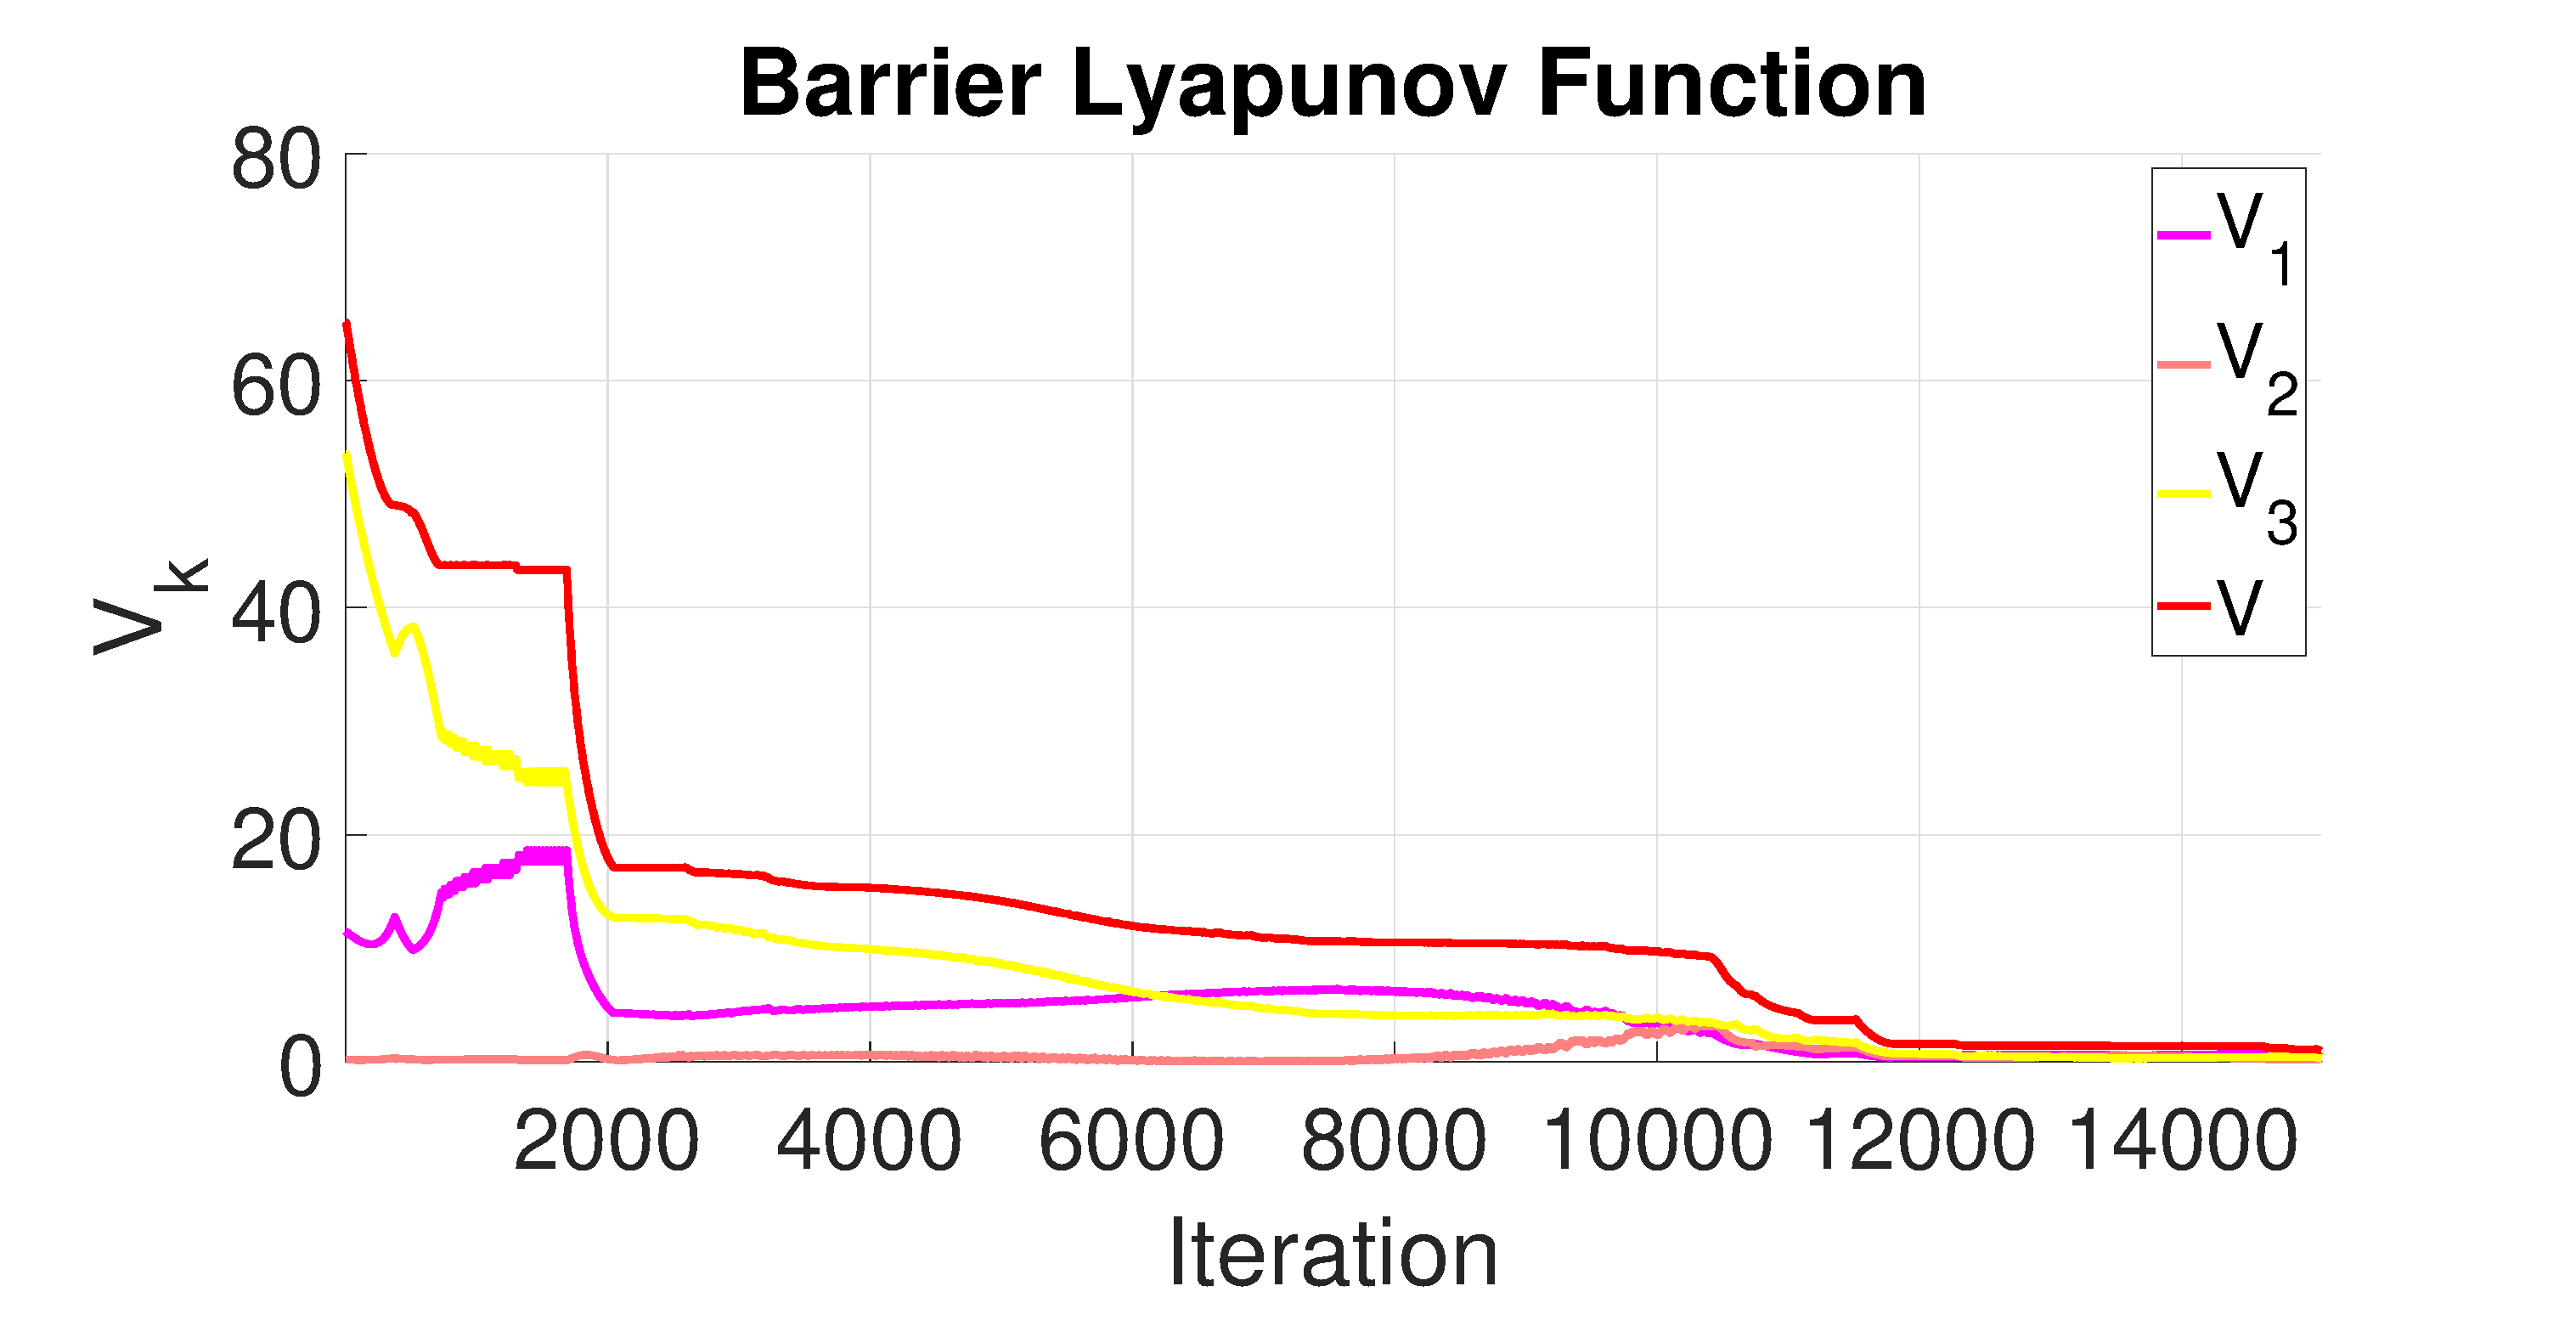
\includegraphics[width=9.6cm]{BLF}
		\caption{Convergence of the non-increasing BLF $V(Z)$ and the sub-BLF of each agent $V_k(Z)$}
		\label{fig:BLF}
	\end{figure}
	
	As can be seen from figure (\ref{fig:BLF}), even though each BLF $V_k$ does not have a non-positive time derivative, they are bounded by $V(Z)$. Figure (\ref{fig:CVT}) depicts the final CVT achieved by the distributed control input. All virtual masses establishes a desired CVT. Furthermore, figure (\ref{fig:vmTraj}) shows the trajectories of the virtual
	masses, which proves that they never cross the boundary lines.
	
	\begin{figure}[H]
		\centering
		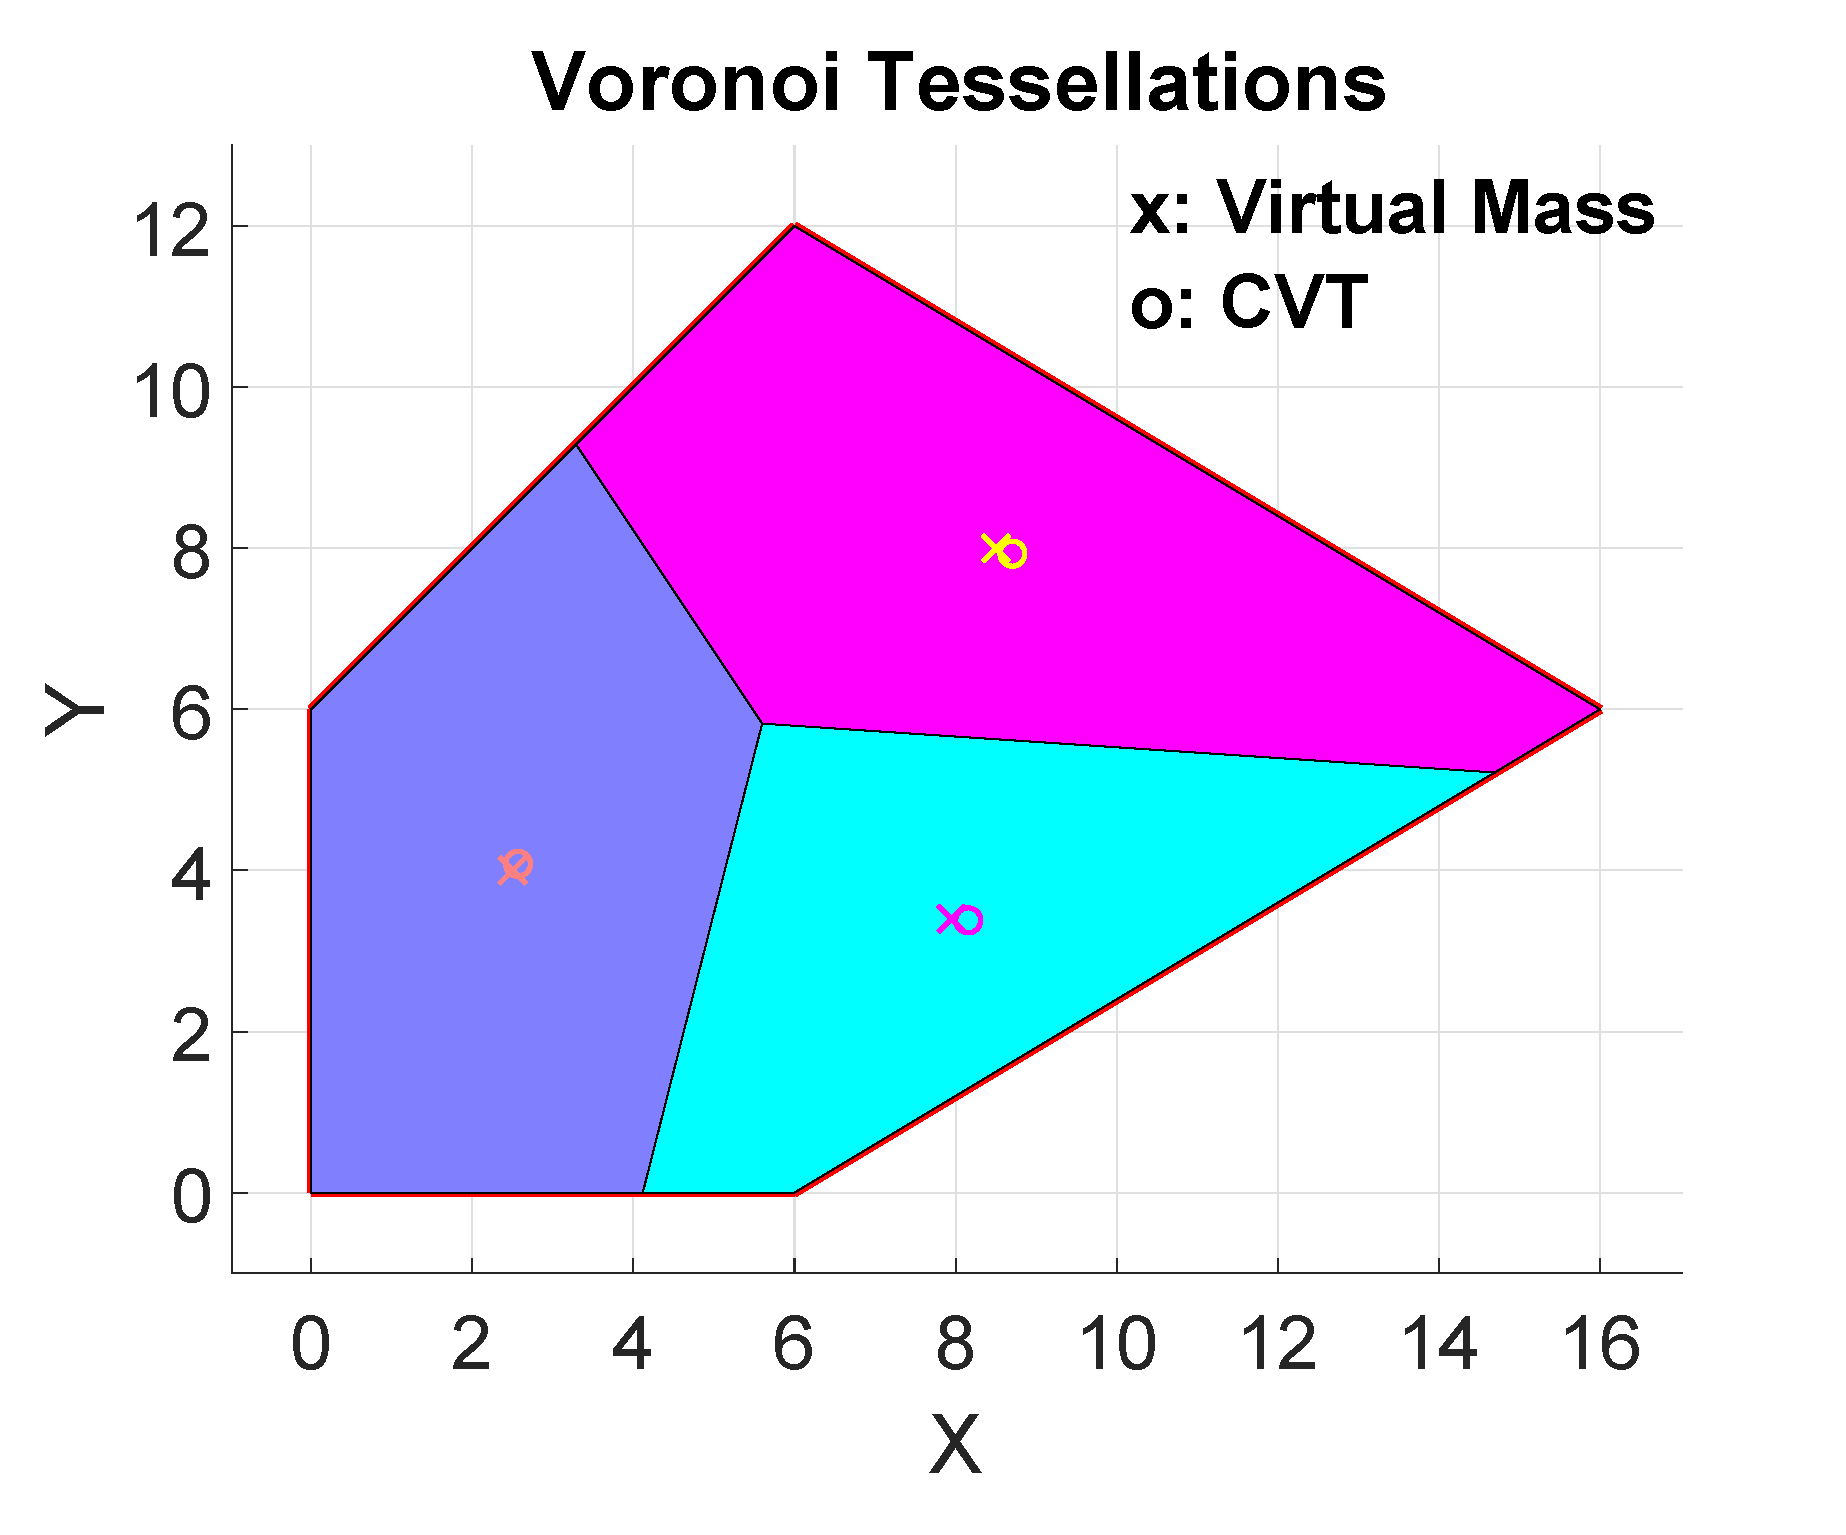
\includegraphics[width=8cm]{Voronoi_Tessellation.eps}
		\caption{Centroidal Voronoi tessellation established by virtual masses}
		\label{fig:CVT}
	\end{figure}
	
	\begin{figure}[H]
		\centering
		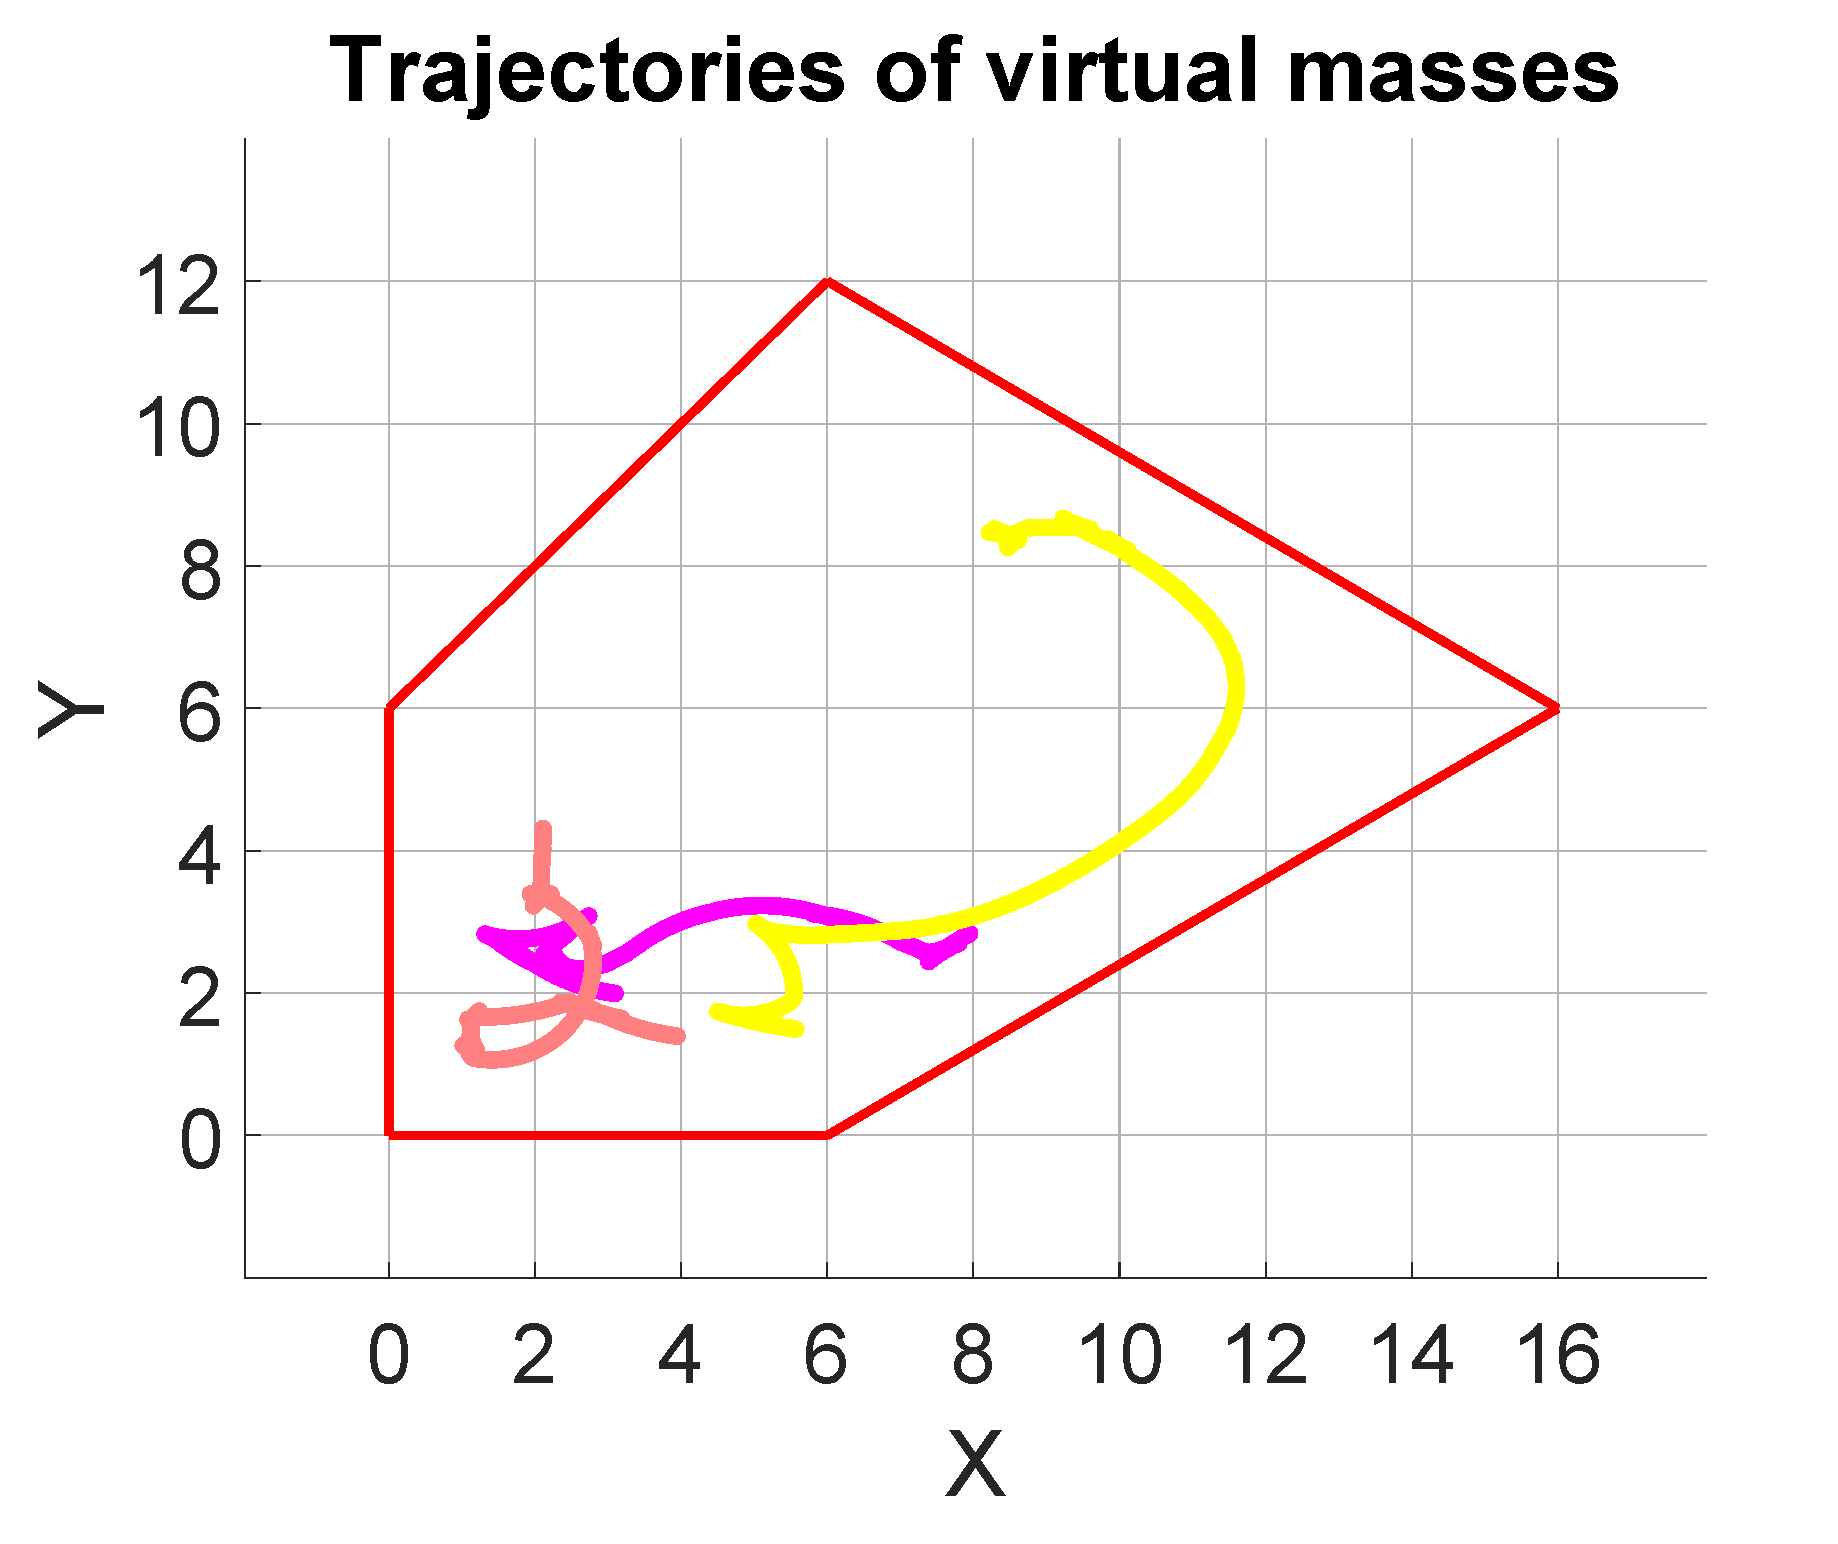
\includegraphics[width=8cm]{VM_Trajectories.eps}
		\caption{Trajectories of virtual masses}
		\label{fig:vmTraj}
	\end{figure}
	
	Figure (\ref{fig:u_k}) shows that the control input of agents are bounded between the predefined maximum angular velocity ($-0.5, 0.5$) rad/s
	
	\begin{figure}[H]
		\centering
		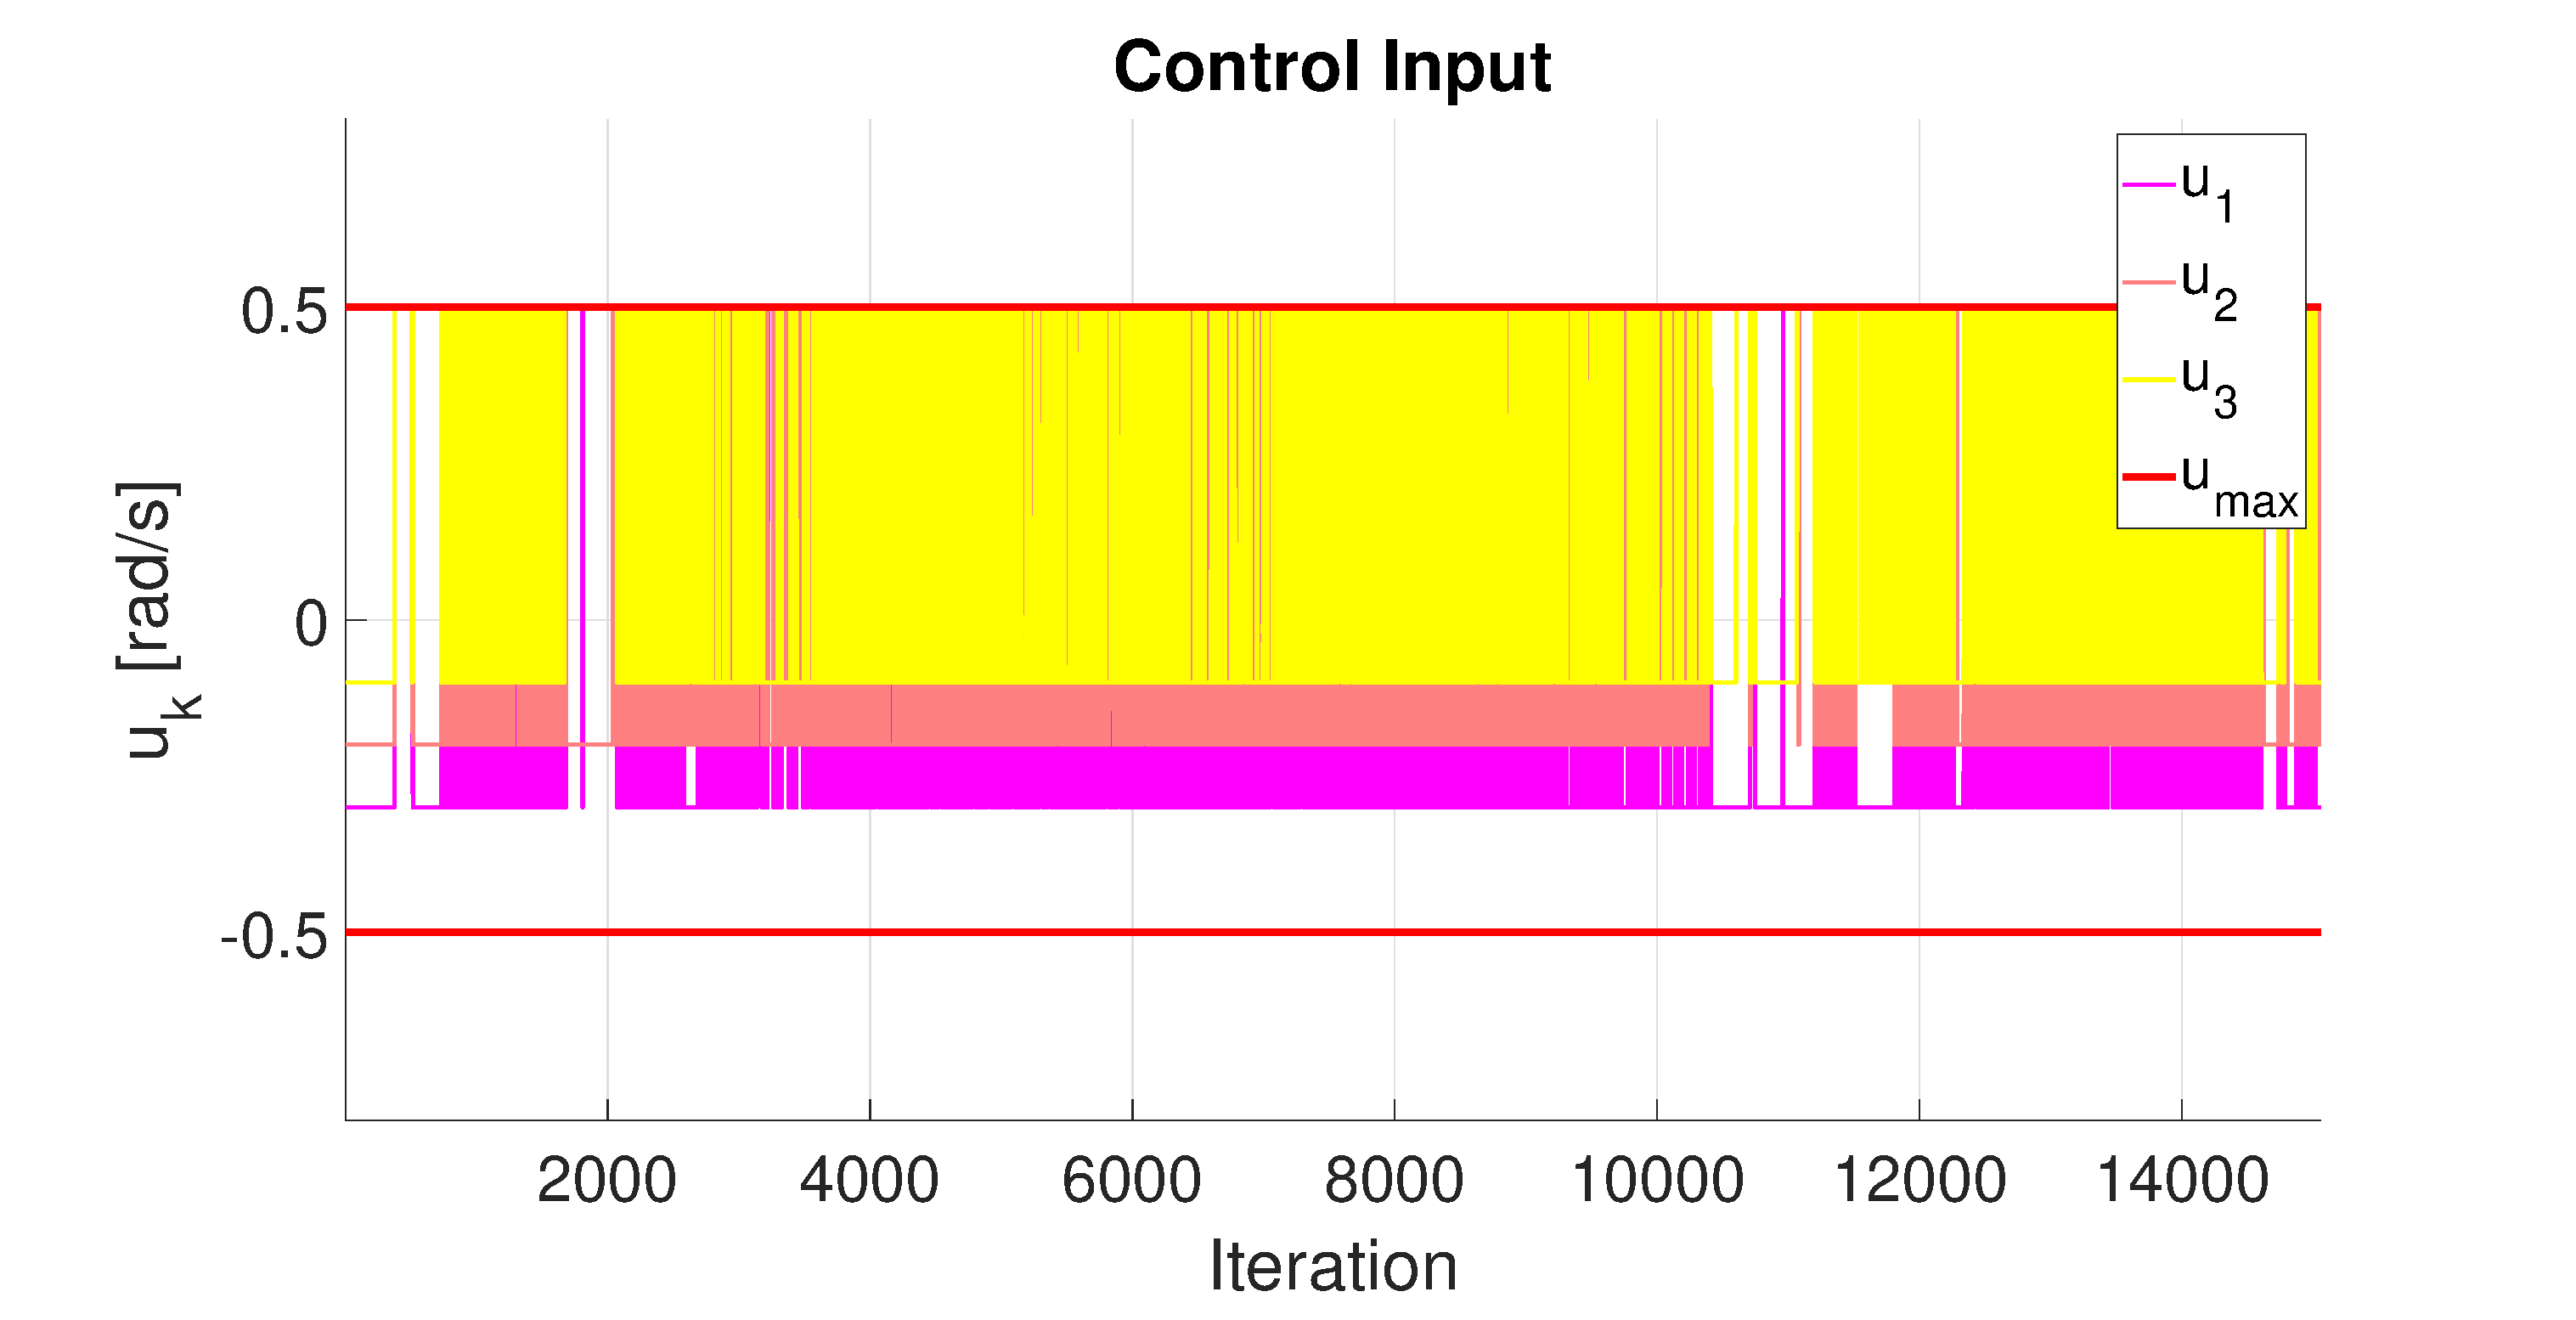
\includegraphics[width=9.6cm]{u_k}
		\caption{Control input of each agent}
		\label{fig:u_k}
	\end{figure}
	%\section{Experimental Validation}
	
	\section{Conclusion} \label{section:conclusion}
	%The conclusion goes here.
	
	\appendices
	\section{Partial derivative of BLF} \label{appendix:BLF}
	\noindent Remind the sub BLF of the adjacent agent $i$ is $V_i(Z): \mathbb{C}^n \rightarrow \mathbb{R}_+$, which is defined as 
	\[V_i(Z) = \sum^{m}_{j=1} \frac{1}{2} \frac{\left< z_i - C_i(Z), z_i - C_i(Z)\right>}{b_j - \left<z_i, a_j \right>}\] \notag
	\noindent In \cite{Du}, Du formulated the term $\frac{\partial C_i}{\partial z_k}$ in $\mathbb{R}^2$ as 
	\begin{equation} 
	\begin{split}
	\frac{\partial {C}^{(a)}_i}{\partial {z_k}^{(b)}} = & \frac{\int_{\partial \Omega_{i,k}} \rho(q)q^{(a)} \frac{q^{(b)} - {z}^{(b)}_k}{\norm{z_k - z_i}} dq}{m_i} \\ 
	& - \frac{(\int_{\partial \Omega_{i,k}} \rho(q)\frac{q^{(b)} - {z_k}^{(b)}}{\norm{z_k - z_i}} dq)(\int_{\Omega_i(Z)}^{} \rho(q)q^{(a)}dq)}{m_i^2} \\
	\end{split}
	\end{equation}
	where 
	\begin{equation}
	\begin{split}
	& a,b \in \{ x,y \}   \\
	& m_i = \int_{\Omega_{i}(Z)}^{} \rho(q)dq \\ 
	\end{split}
	\end{equation}
	Note that in the introduced BLF $V_{i}(Z)$, even though the term $C_{i}(Z)$ are defined in the complex domain, its partial derivative $\frac{\partial C_i}{\partial z_k}$ is computed in the real planar as a Jacobian matrix 
	%By using the above equation, the obtained $\frac{\partial C_i}{\partial z_k}$ is represented as a Jacobian matrix in $\mathbb{R}^2$, which is
	\begin{equation} \label{eqn:dVidz}
	\begin{split}
	\frac{\partial C_i}{\partial z_k} = \left [\begin{matrix}
	\frac{\partial C_{ix}}{\partial z_{kx}} & \frac{\partial C_{ix}}{\partial z_{ky}}   \\
	\frac{\partial C_{iy}}{\partial z_{kx}} & \frac{\partial C_{iy}}{\partial z_{ky}} \\
	\end{matrix} \right ] \in \mathbb{R}^2
	\end{split}
	\end{equation}
	where 
	\begin{equation} \label{eqn:dVidz}
	\begin{split}
	C_i & = [C_{ix}, C_{iy}]^T \\
	z_k & = [z_{kx}, z_{ky}]^T \\
	\end{split}
	\end{equation}
	
	
	It is concluded that the partial derivative of $C_i(Z)$ does not depend on the non-adjacent agent, this implies 
	\begin{equation} \label{eqn:dVidz}
	\begin{split}
	\frac{\partial C_i}{\partial z_k} = \threepartdef	{\frac{\partial C_k}{\partial z_k}}			{i = k}
	{\frac{\partial C_i}{\partial z_k}}			{i \in \tilde{K}}
	{0}											{i \notin \tilde{K}} 												
	\end{split}
	\end{equation}
	
	
	Furthermore, the above-mentioned Jacobian matrix will occur in the inner product as a result of the applied derivation rule 
	\[\frac{d}{dz}\left < f,g\right > = \left < \frac{d}{dz}f, g \right > + \left < f, \frac{d}{dz} g \right >\]
	In order to strictly follow the definition of the inner product, we introduce the new opearator $\odot: \mathbb{R}^{2 \times 2} \times \mathbb{C} \rightarrow \mathbb{C}$ to represent the intuitive meaning of partial derivative in $\mathbb{C}$ plane
	\[\left < A \odot z\right > = A \begin{bmatrix}
	\Re (z) \\
	\Im (z) \\
	\end{bmatrix} \]   
	where the right equation is the matrix multiplication between $A \in \mathbb{R}^{2\times2}$ and a vector in $\mathbb{R}^2$. The partial derivative of $V_i(Z)$ is then computed as
	\begin{itemize} [leftmargin=*]
		\item $ i = k $
		\begin{equation} \notag
		\begin{split}
		\frac{\partial V_k(Z)}{\partial z_k} & = \left<I_{2 \times 2} -\frac{\partial C_k(Z)}{\partial z_k} \odot z_k - C_k(Z)\right>     \sum^{m}_{j=1} \frac{1}{b_j - \left<z_k, a_j \right> } \\
		& - \frac{\left< z_k - C_k(Z), z_k - C_k(Z)\right>}{2} 					\sum^{m}_{j=1} \frac{a_j}{\left (b_j - \left<z_k, a_j \right>\right )^2} 
		\end{split}
		\end{equation}
		\text{Note: $I_{2 \times 2}$ is the identity matrix}
		
		\item $ i \in \tilde{K} $
		\[\frac{\partial V_i(Z)}{\partial z_k} = \left<- \frac{\partial C_i(Z)}{\partial z_k} \odot z_i - C_i(Z)\right>     \sum^{m}_{j=1} \frac{1}{b_j - \left<z_i, a_j \right> }\]
		
		\item $ i \notin \tilde{K} $
		\[\frac{\partial V_i(Z)}{\partial z_k} = 0 \]
		
	\end{itemize}
	
	It is concluded that the term $V_i(Z)$ does not depend on the non-adjacent agent, which allow each agent to compute from the limited information of the adjacent within the communication range.
	
	%****************** Partial derivative of BLF ****************** \\
	%FIRST MULTIPLICAND
	%\begin{equation} \label{eqn:distance_der}
	%\begin{split}
	%& \frac{\partial}{\partial z_k} \left< z_i - C_i(Z), z_i - C_i(Z)\right>  \\
	%& = 2 \left<\frac{\partial}{\partial z_k} (z_i - C_i(Z)), z_i - C_i(Z)\right> \\
	%& = \threepartdef 	{2 \left<1 - \frac{\partial C_i(Z)}{\partial z_k}, z_i - C_i(Z)\right>}				{i = k}	
	%{2 \left<- \frac{\partial C_i(Z)}{\partial z_k}, z_i - C_i(Z)\right>}					{i \in \tilde{K}}
	%{0}																					{i \notin \tilde{K}}
	%\end{split}
	%\end{equation}
	%SECOND MULTIPLICAND
	%\begin{equation} \label{eqn:guard_doc}
	%\begin{split}
	%& \frac{\partial}{\partial z_k} \left ( \sum^{m}_{j=1} \frac{1}{b_j - \left<z_i, a_j \right> } \right)  \\
	%& = \twopartdef 	{- \sum^{m}_{j=1} \frac{a_j}{\left (b_j - \left<z_i, a_j \right> \right )^2} }		{i = k}	
	%{0}																					{i \neq k}
	%\end{split}
	%\end{equation}
	
	%Together
	%\begin{equation} \label{eqn:Vk_dot_implementation}
	%\begin{split}
	%& \frac{\partial V_i(Z)}{\partial z_k} \\
	%& = \frac{\partial}{\partial z_k} \left ( \sum^{m}_{j=1} \frac{1}{2} \frac{\left< z_i - C_i(Z), z_i - %C_i(Z)\right>}{b_j -\left<z_i, a_j \right> } \right) \\ % Partial BLF of each agent
	%& = \frac{\partial}{\partial z_k} \left (\frac{1}{2} \left< z_i - C_i(Z), z_i - C_i(Z)\right> \sum^{m}_{j=1} \frac{1}{ %b_j -\left<z_i, a_j \right>} \right) \\
	%& = \left < \frac{\partial z_i}{\partial z_k} - \frac{\partial C_i(Z)}{\partial z_k},   z_i - C_i(Z) \right > %\sum^{m}_{j=1} \frac{1}{b_j - \left<z_i, a_j \right>} \\
	%& - ...
	%\end{split}
	%\end{equation}
	% Parital derivative of Vk ************************
	
	
	% An example of a floating figure using the graphicx package.
	% Note that \label must occur AFTER (or within) \caption.
	% For figures, \caption should occur after the \includegraphics.
	% Note that IEEEtran v1.7 and later has special internal code that
	% is designed to preserve the operation of \label within \caption
	% even when the captionsoff option is in effect. However, because
	% of issues like this, it may be the safest practice to put all your
	% \label just after \caption rather than within \caption{}.
	%
	% Reminder: the "draftcls" or "draftclsnofoot", not "draft", class
	% option should be used if it is desired that the figures are to be
	% displayed while in draft mode.
	%
	%\begin{figure}[!t]
	%\centering
	%\includegraphics[width=2.5in]{myfigure}
	% where an .eps filename suffix will be assumed under latex, 
	% and a .pdf suffix will be assumed for pdflatex; or what has been declared
	% via \DeclareGraphicsExtensions.
	%\caption{Simulation results for the network.}
	%\label{fig_sim}
	%\end{figure}
	
	% Note that the IEEE typically puts floats only at the top, even when this
	% results in a large percentage of a column being occupied by floats.
	
	
	% An example of a double column floating figure using two subfigures.
	% (The subfig.sty package must be loaded for this to work.)
	% The subfigure \label commands are set within each subfloat command,
	% and the \label for the overall figure must come after \caption.
	% \hfil is used as a separator to get equal spacing.
	% Watch out that the combined width of all the subfigures on a 
	% line do not exceed the text width or a line break will occur.
	%
	%\begin{figure*}[!t]
	%\centering
	%\subfloat[Case I]{\includegraphics[width=2.5in]{box}%
	%\label{fig_first_case}}
	%\hfil
	%\subfloat[Case II]{\includegraphics[width=2.5in]{box}%
	%\label{fig_second_case}}
	%\caption{Simulation results for the network.}
	%\label{fig_sim}
	%\end{figure*}
	%
	% Note that often IEEE papers with subfigures do not employ subfigure
	% captions (using the optional argument to \subfloat[]), but instead will
	% reference/describe all of them (a), (b), etc., within the main caption.
	% Be aware that for subfig.sty to generate the (a), (b), etc., subfigure
	% labels, the optional argument to \subfloat must be present. If a
	% subcaption is not desired, just leave its contents blank,
	% e.g., \subfloat[].
	
	
	% An example of a floating table. Note that, for IEEE style tables, the
	% \caption command should come BEFORE the table and, given that table
	% captions serve much like titles, are usually capitalized except for words
	% such as a, an, and, as, at, but, by, for, in, nor, of, on, or, the, to
	% and up, which are usually not capitalized unless they are the first or
	% last word of the caption. Table text will default to \footnotesize as
	% the IEEE normally uses this smaller font for tables.
	% The \label must come after \caption as always.
	%
	%\begin{table}[!t]
	%% increase table row spacing, adjust to taste
	%\renewcommand{\arraystretch}{1.3}
	% if using array.sty, it might be a good idea to tweak the value of
	% \extrarowheight as needed to properly center the text within the cells
	%\caption{An Example of a Table}
	%\label{table_example}
	%\centering
	%% Some packages, such as MDW tools, offer better commands for making tables
	%% than the plain LaTeX2e tabular which is used here.
	%\begin{tabular}{|c||c|}
	%\hline
	%One & Two\\
	%\hline
	%Three & Four\\
	%\hline
	%\end{tabular}
	%\end{table}
	
	
	% Note that the IEEE does not put floats in the very first column
	% - or typically anywhere on the first page for that matter. Also,
	% in-text middle ("here") positioning is typically not used, but it
	% is allowed and encouraged for Computer Society conferences (but
	% not Computer Society journals). Most IEEE journals/conferences use
	% top floats exclusively. 
	% Note that, LaTeX2e, unlike IEEE journals/conferences, places
	% footnotes above bottom floats. This can be corrected via the
	% \fnbelowfloat command of the stfloats package.
	
	
	
	% if have a single appendix:
	%\appendix[Proof of the Zonklar Equations]
	% or
	%\appendix  % for no appendix heading
	% do not use \section anymore after \appendix, only \section*
	% is possibly needed
	
	% use appendices with more than one appendix
	% then use \section to start each appendix
	% you must declare a \section before using any
	% \subsection or using \label (\appendices by itself
	% starts a section numbered zero.)
	%
	
	% use section* for acknowledgment
	\section*{Acknowledgment}
	
	
	The authors would like to thank...
	
	
	% Can use something like this to put references on a page
	% by themselves when using endfloat and the captionsoff option.
	\ifCLASSOPTIONcaptionsoff
	\newpage
	\fi
	
	
	
	% trigger a \newpage just before the given reference
	% number - used to balance the columns on the last page
	% adjust value as needed - may need to be readjusted if
	% the document is modified later
	%\IEEEtriggeratref{8}
	% The "triggered" command can be changed if desired:
	%\IEEEtriggercmd{\enlargethispage{-5in}}
	
	% references section
	
	% can use a bibliography generated by BibTeX as a .bbl file
	% BibTeX documentation can be easily obtained at:
	% http://mirror.ctan.org/biblio/bibtex/contrib/doc/
	% The IEEEtran BibTeX style support page is at:
	% http://www.michaelshell.org/tex/ieeetran/bibtex/
	%\bibliographystyle{IEEEtran}
	% argument is your BibTeX string definitions and bibliography database(s)
	%\bibliography{IEEEabrv,../bib/paper}
	%
	% <OR> manually copy in the resultant .bbl file
	% set second argument of \begin to the number of references
	% (used to reserve space for the reference number labels box)
	\begin{thebibliography}{1}
		
		%\bibitem{IEEEhowto:kopka}
		%H.~Kopka and P.~W. Daly, \emph{A Guide to \LaTeX}, 3rd~ed.\hskip 1em plus
		%0.5em minus 0.4em\relax Harlow, England: Addison-Wesley, 1999.
		\bibitem{Cortes}
		Jorge Cortes, Sonia Martinez, Timur Karatas, Francesco Bullo and \textit{Member IEEE}.
		\emph{Coverage control for mobile sensing networks}. 
		IEEE Transactions on Robotics and Automation.
		
		\bibitem{Schwager}
		Mac Schwager.
		\emph{A Gradient Optimization Approach to Adaptive Multi-Robot Control}. 
		Ph.D. thesis, Massachusetts Institute of Technology.
		
		%\bibitem{Schwager2}
		%\emph{Distributed Coverage Control with Sensory Feedback for Networked Robots}
		%Mac Schwager, James McLurkin, and Daniela Rus
		
		\bibitem{Qingchen} 
		Qingchen Liu, Mengbin Ye, Zhiyong Sun, Jiahu Qin, and Changbin Yu.
		\emph{Coverage control of unicycle agents under constant speed constraints}. 
		IFAC-PapersOnLine, 50(1):2471{2476, 2017}.
		
		\bibitem{DistributedGraph}
		Christoforos N Hadjicostis and Min Cao. \emph{Distributed algorithms for Voronoi diagrams and applications in ad-hoc networks} Technical report, Coordinated Science Laboratory, University of Illinois at Urbana-Champaign, 2003.
		
		\bibitem{MDV}
		Matthew L. Elwin, Randy A. Freeman, and Kevin M. Lynch. \emph{Distributed Voronoi Neighbor Identification From
			Inter-Robot Distances} IEEE ROBOTICS AND AUTOMATION LETTERS, VOL. 2, NO. 3, JULY 2017
		
		\bibitem{Tee}
		Keng Peng Tee, Shuzhi Sam Gea, Eng Hock Tay.
		\emph{Barrier Lyapunov Functions for the control of output-constrained nonlinear systems}
		Automatica, Volume 45, Issue 4, 2009, Pages 918-927, ISSN 0005-1098, https://doi.org/10.1016/j.automatica.2008.11.017.
		
		\bibitem{Du}
		Qiang Du and Maria Emelianenko2.
		\emph{Acceleration Schemes for Computing Centroidal Voronoi Tessellations}. 
		Numerical Linear Algebra with Applications. Numer. Linear Algebra Appl. 2006, 13 173 - 192
	\end{thebibliography}
	
	% biography section
	% 
	% If you have an EPS/PDF photo (graphicx package needed) extra braces are
	% needed around the contents of the optional argument to biography to prevent
	% the LaTeX parser from getting confused when it sees the complicated
	% \includegraphics command within an optional argument. (You could create
	% your own custom macro containing the \includegraphics command to make things
	% simpler here.)
	%\begin{IEEEbiography}[{\includegraphics[width=1in,height=1.25in,clip,keepaspectratio]{mshell}}]{Michael Shell}
	% or if you just want to reserve a space for a photo:
	
	\begin{IEEEbiography}{Michael Shell}
		Biography text here.
	\end{IEEEbiography}
	
	% if you will not have a photo at all:
	\begin{IEEEbiographynophoto}{John Doe}
		Biography text here.
	\end{IEEEbiographynophoto}
	
	% insert where needed to balance the two columns on the last page with
	% biographies
	%\newpage
	
	\begin{IEEEbiographynophoto}{Jane Doe}
		Biography text here.
	\end{IEEEbiographynophoto}
	
	% You can push biographies down or up by placing
	% a \vfill before or after them. The appropriate
	% use of \vfill depends on what kind of text is
	% on the last page and whether or not the columns
	% are being equalized.
	
	%\vfill
	
	% Can be used to pull up biographies so that the bottom of the last one
	% is flush with the other column.
	%\enlargethispage{-5in}
	
	
	
	% that's all folks
\end{document}


